\chapter{User Interface Design}

\section{Mockups}
The user can access or register to the application using a Web Interface. The Mockups of the interface 
are shown in the following figures.\\
\begin{figure}[H]
    \centering
    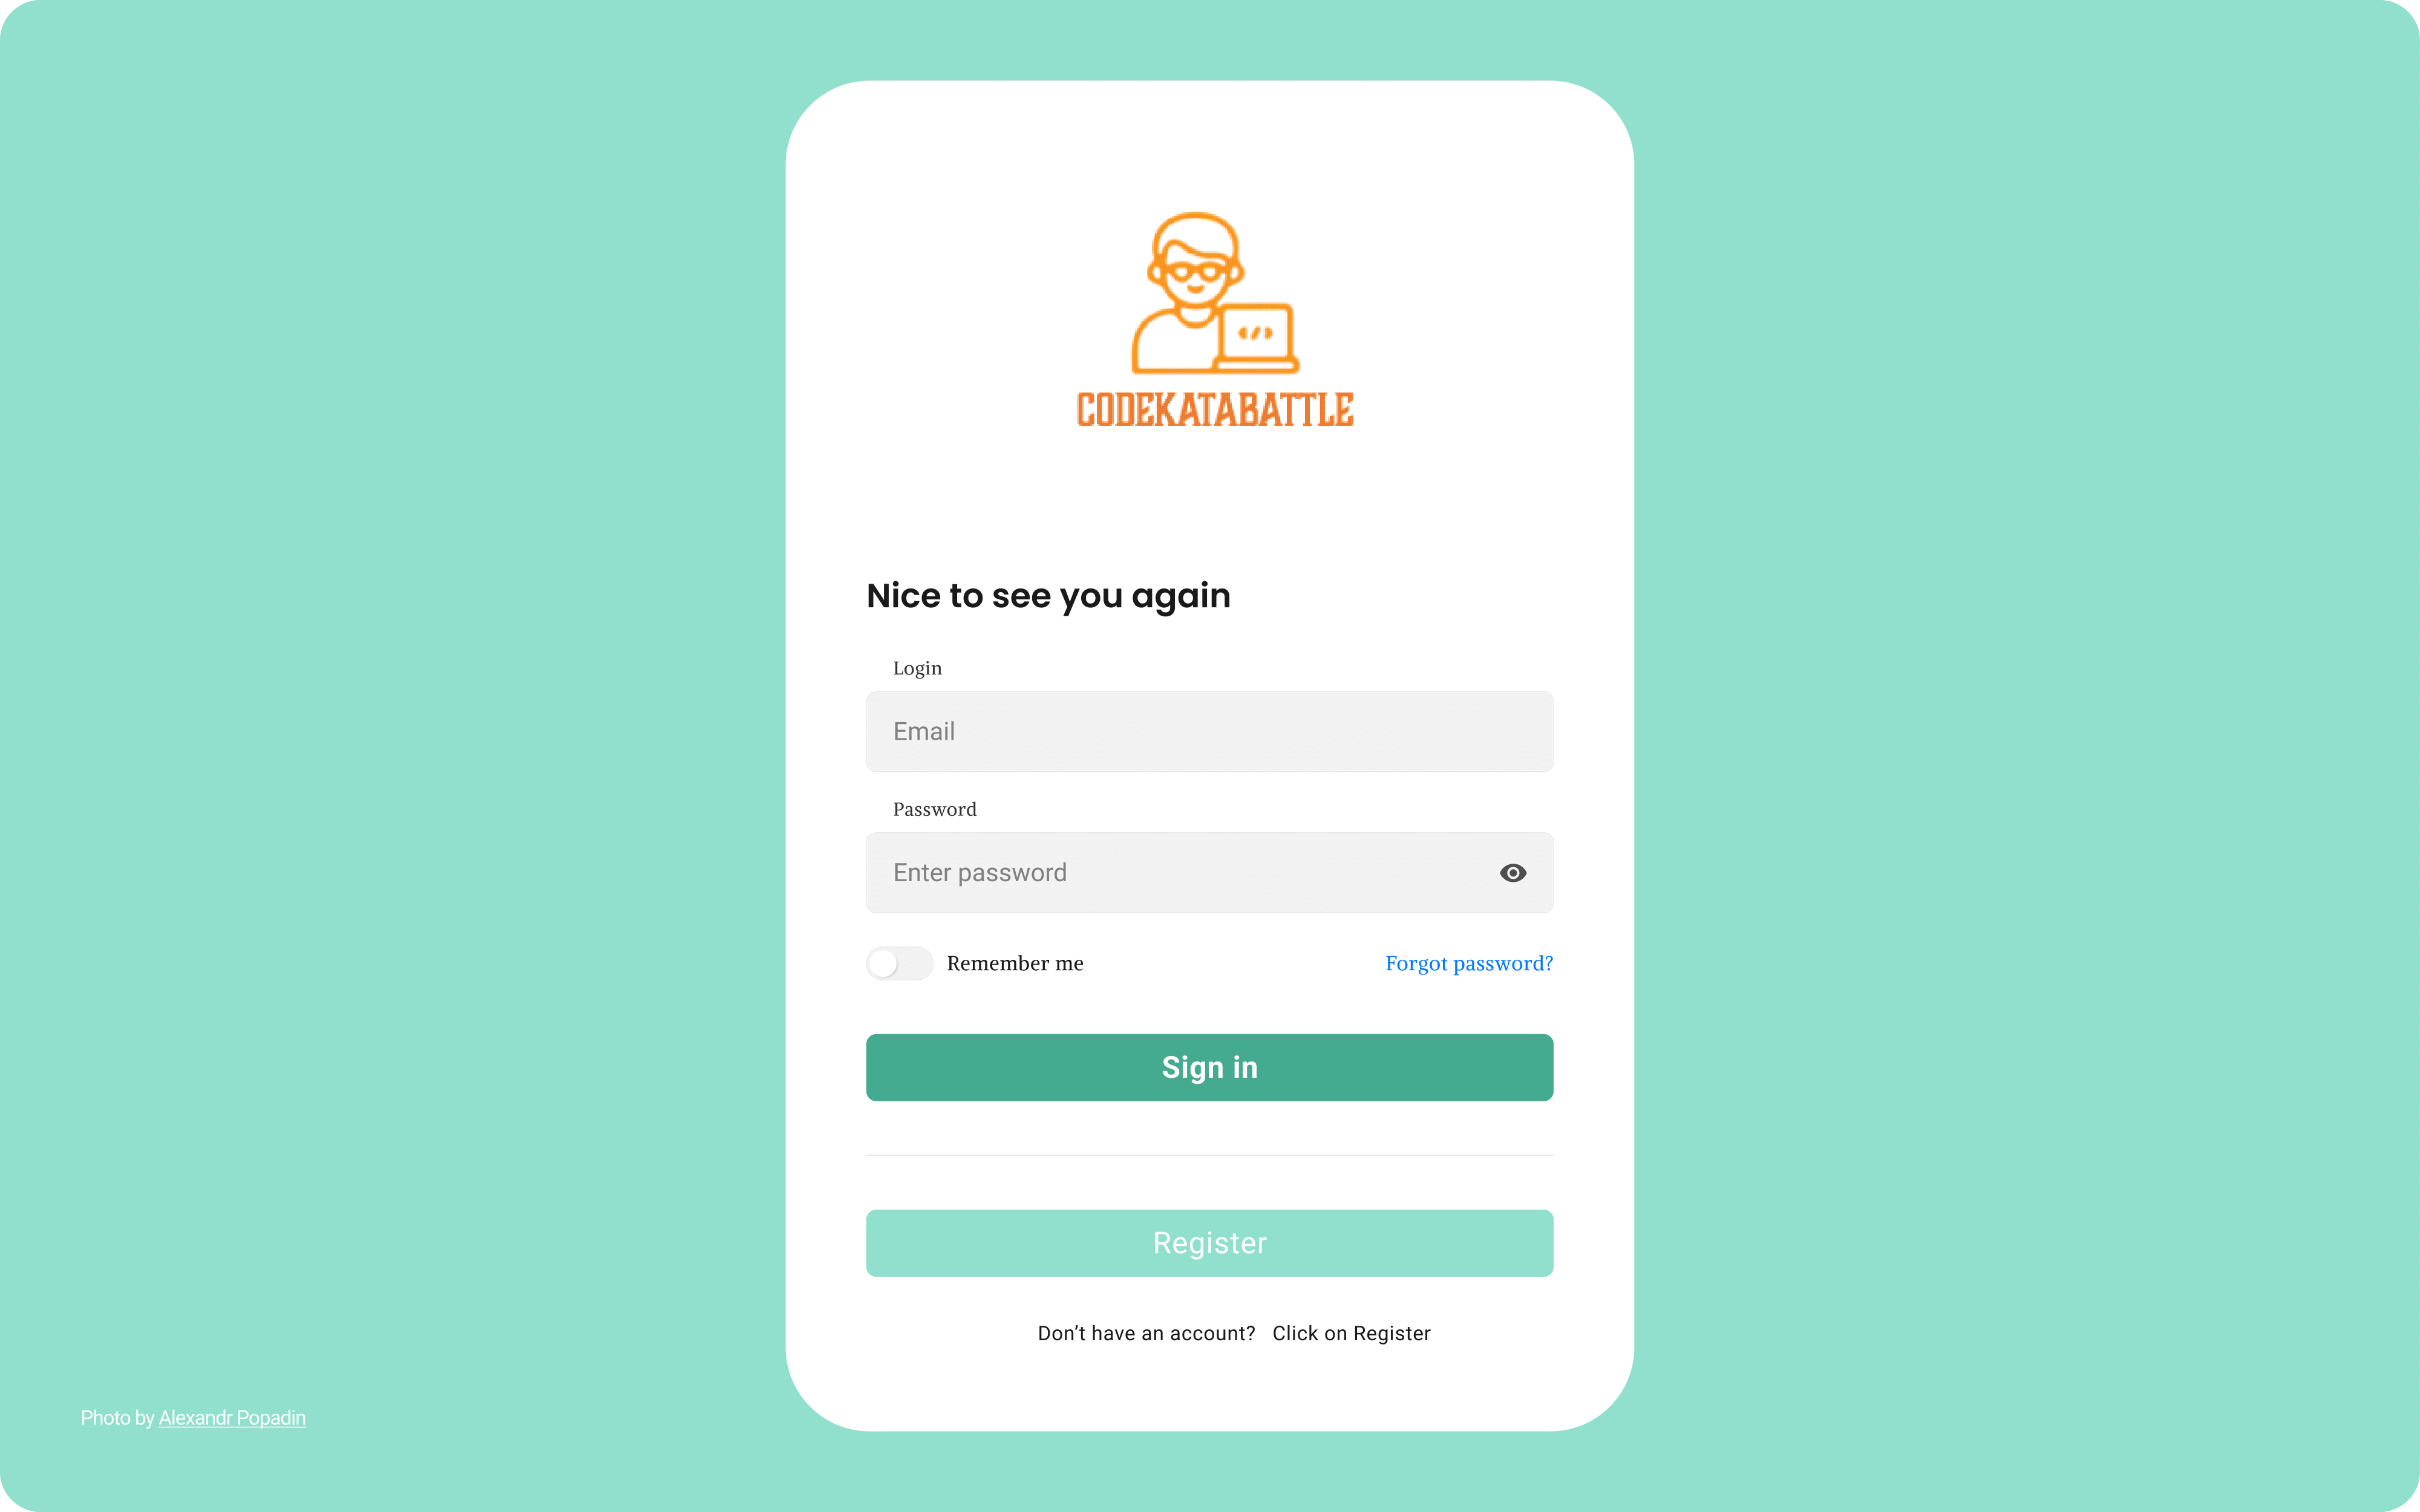
\includegraphics[width=0.8\textwidth]{images/user_interface/UI_sw2-01.png}
    \caption{Login page - same for all types of users}
\end{figure}

\begin{figure}[H]
    \centering
    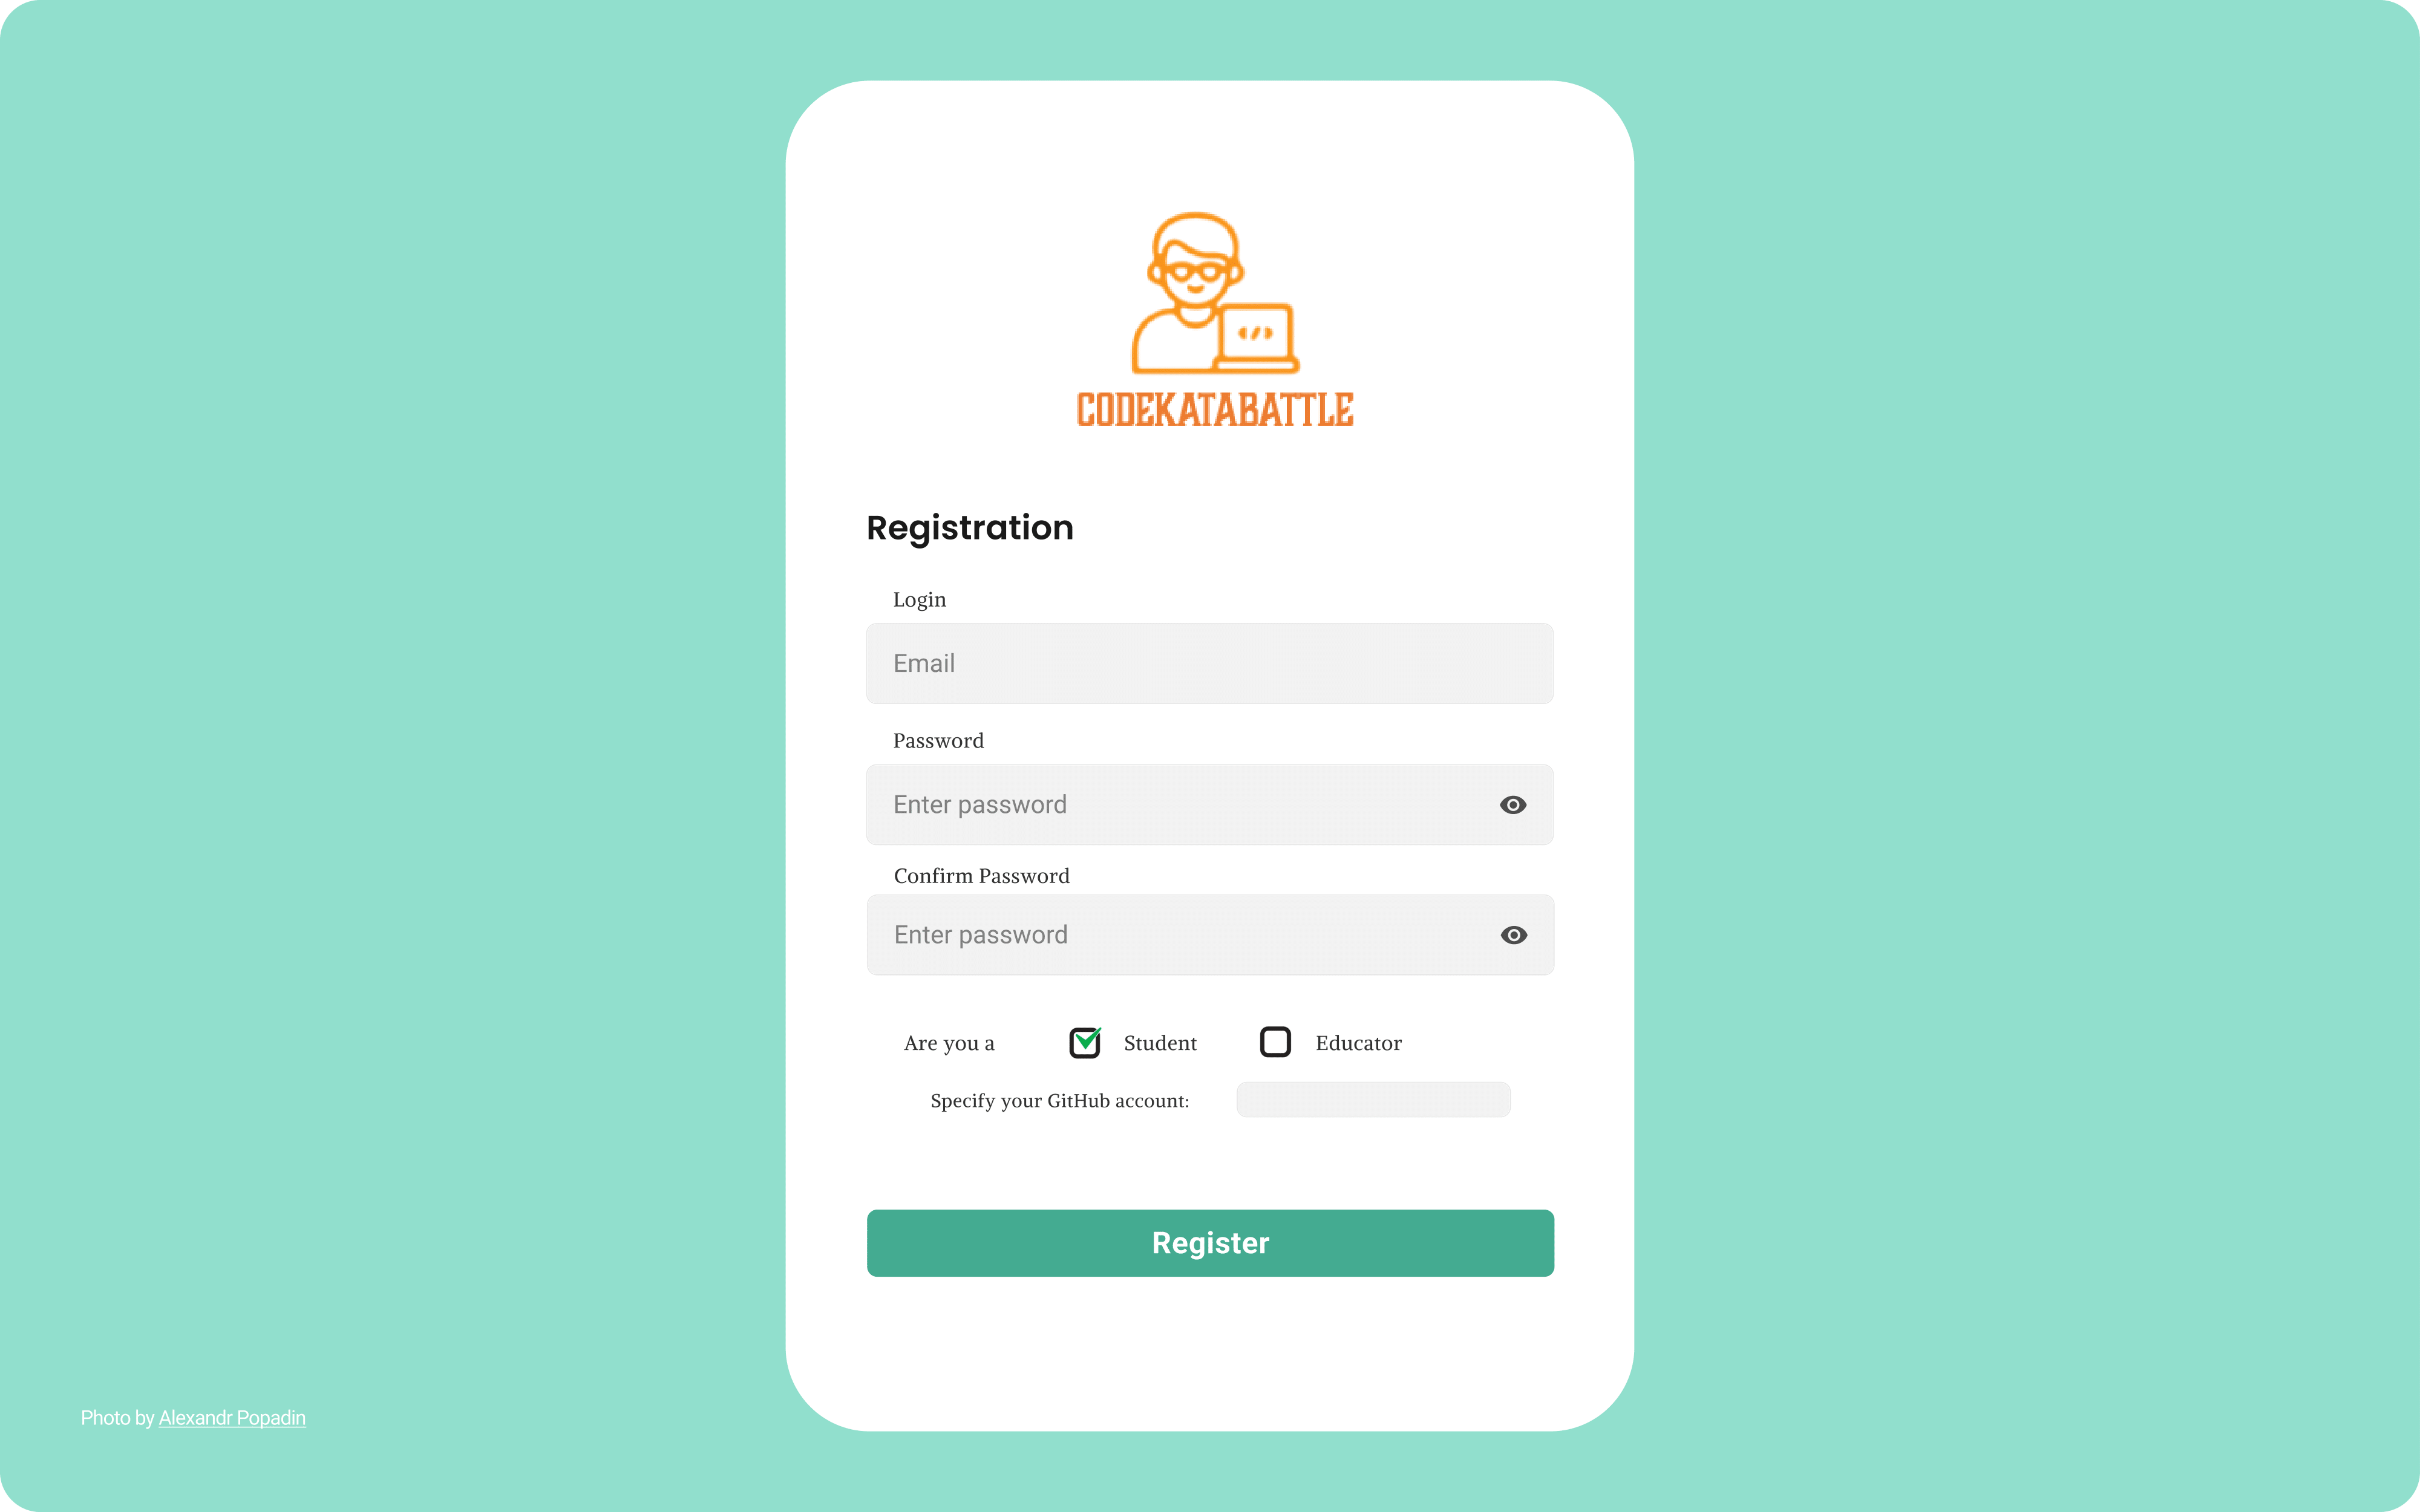
\includegraphics[width=0.8\textwidth]{images/user_interface/UI_sw2-02.png}
    \caption{Registration page - same for all types of users}
\end{figure}

\begin{figure}[H]
    \centering
    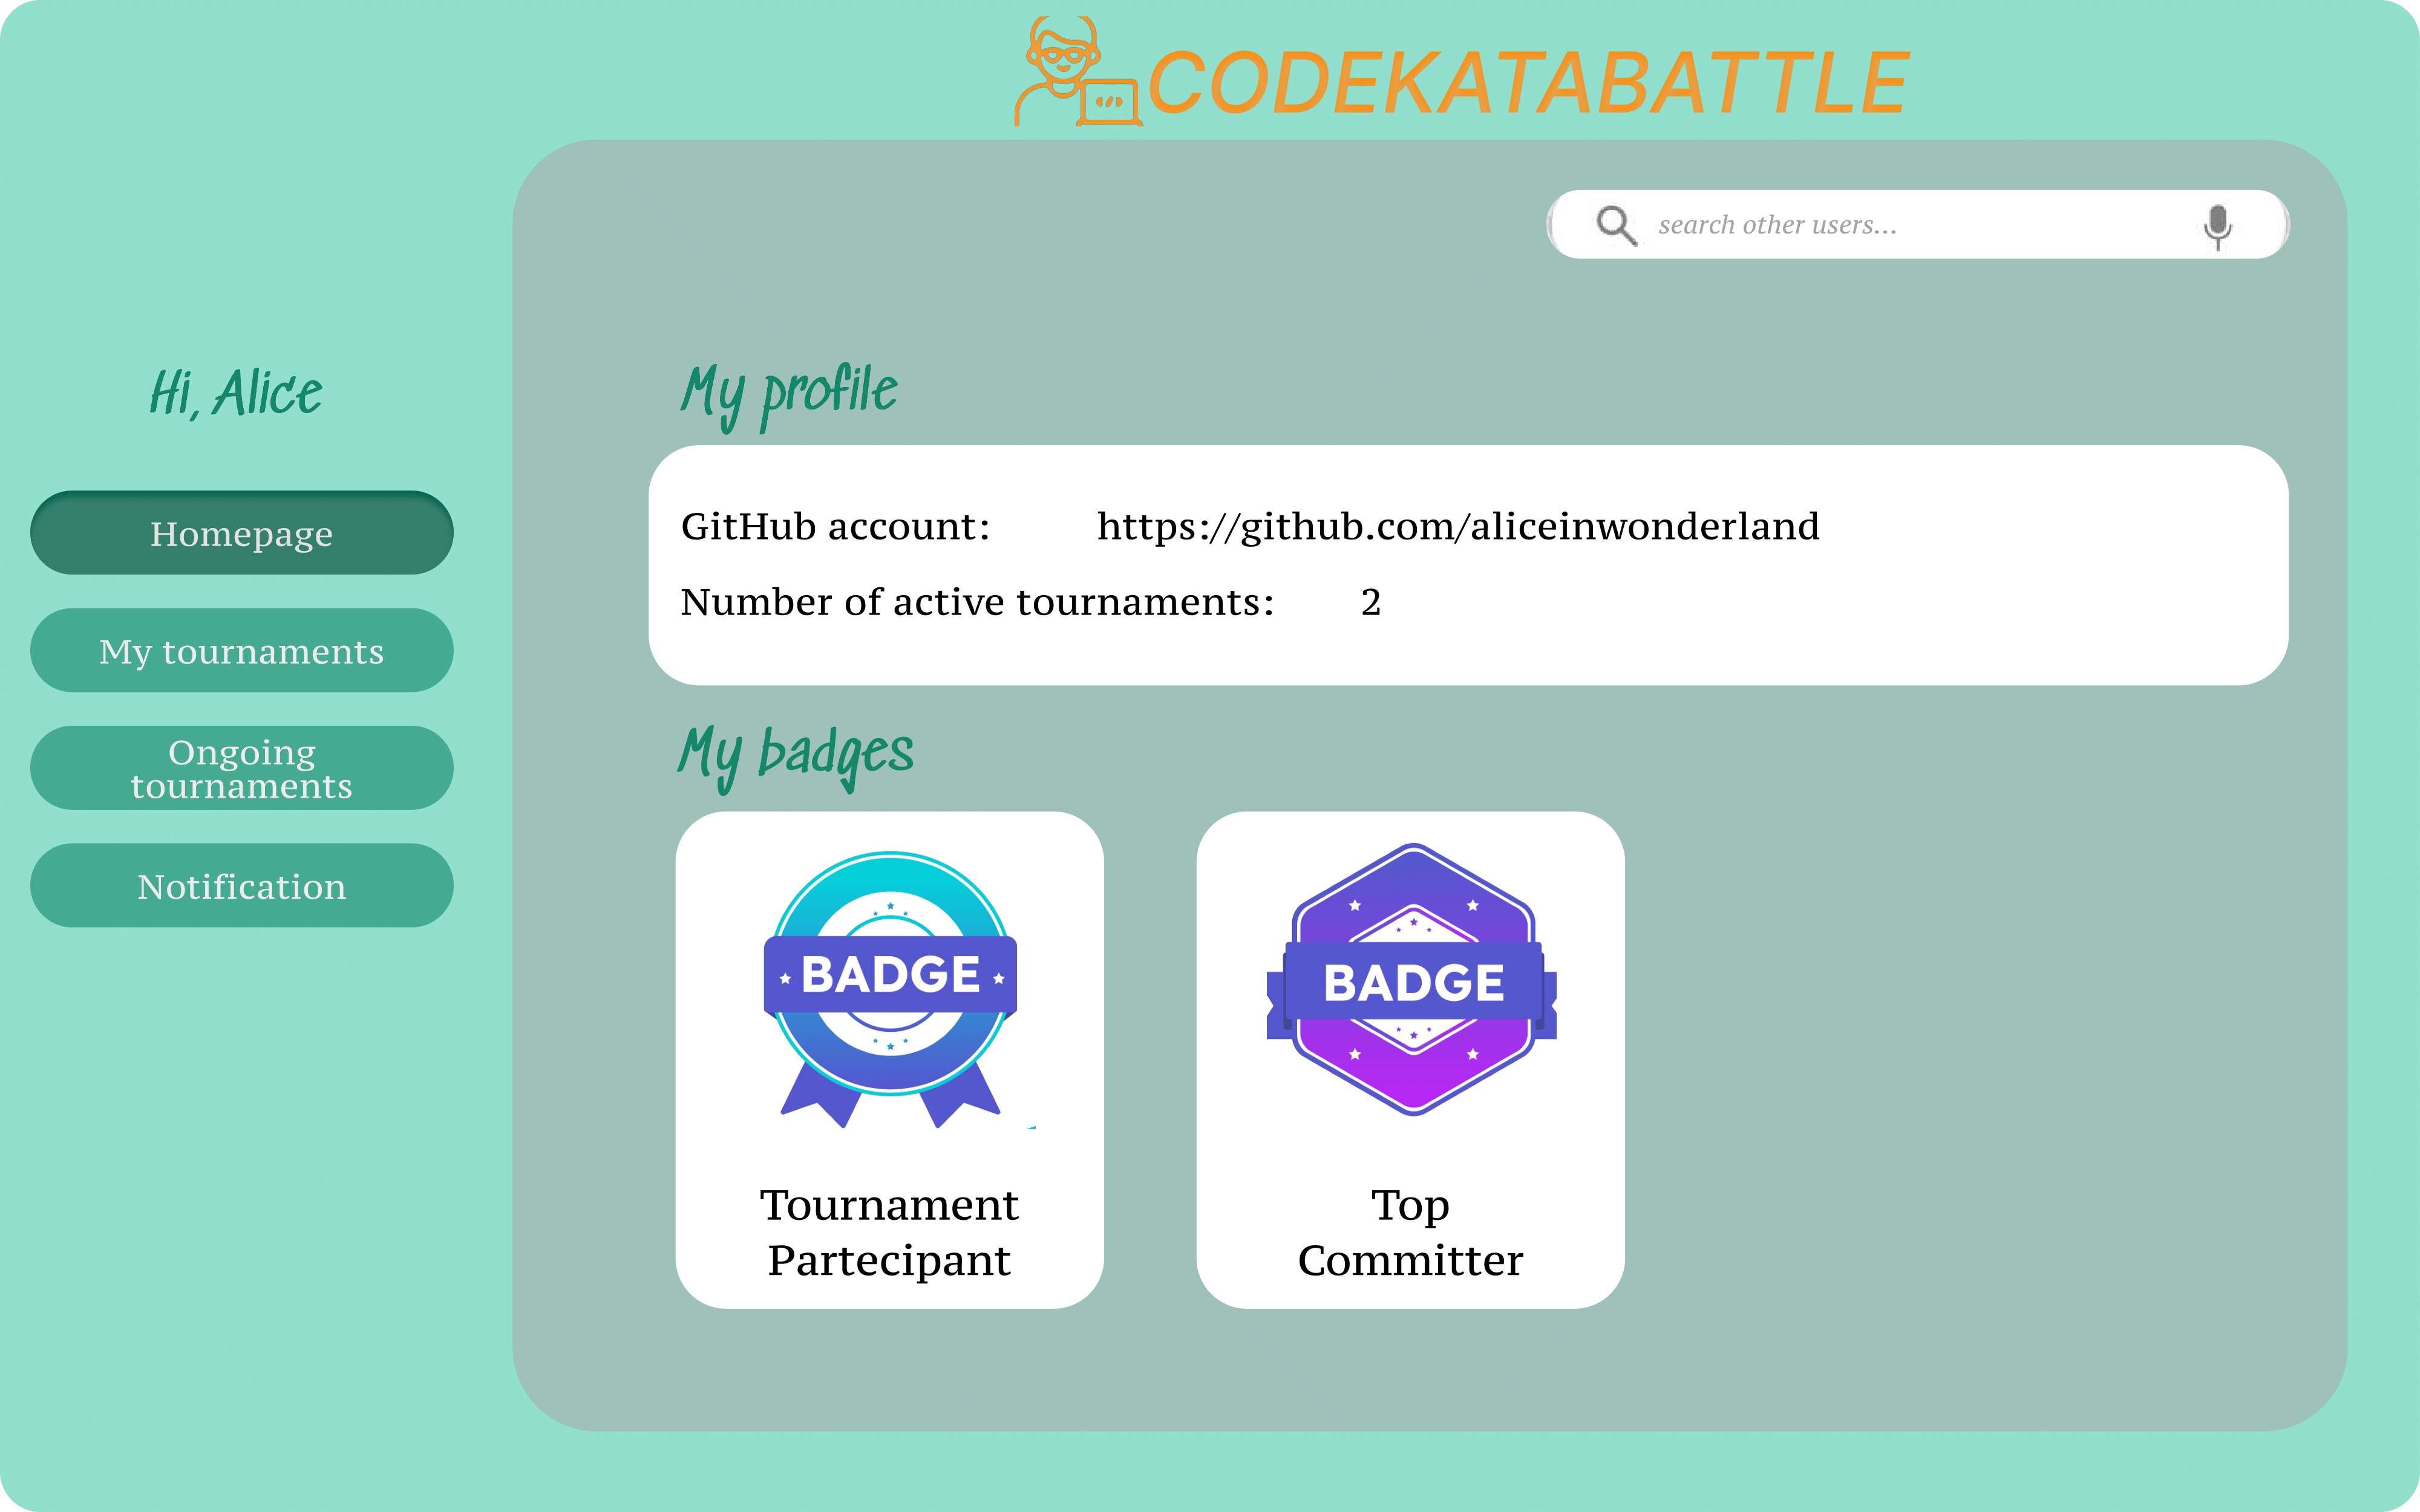
\includegraphics[width=0.8\textwidth]{images/user_interface/UI_sw2-03.png}
    \caption{Student's homepage and profile}
\end{figure}

\begin{figure}[H]
    \centering
    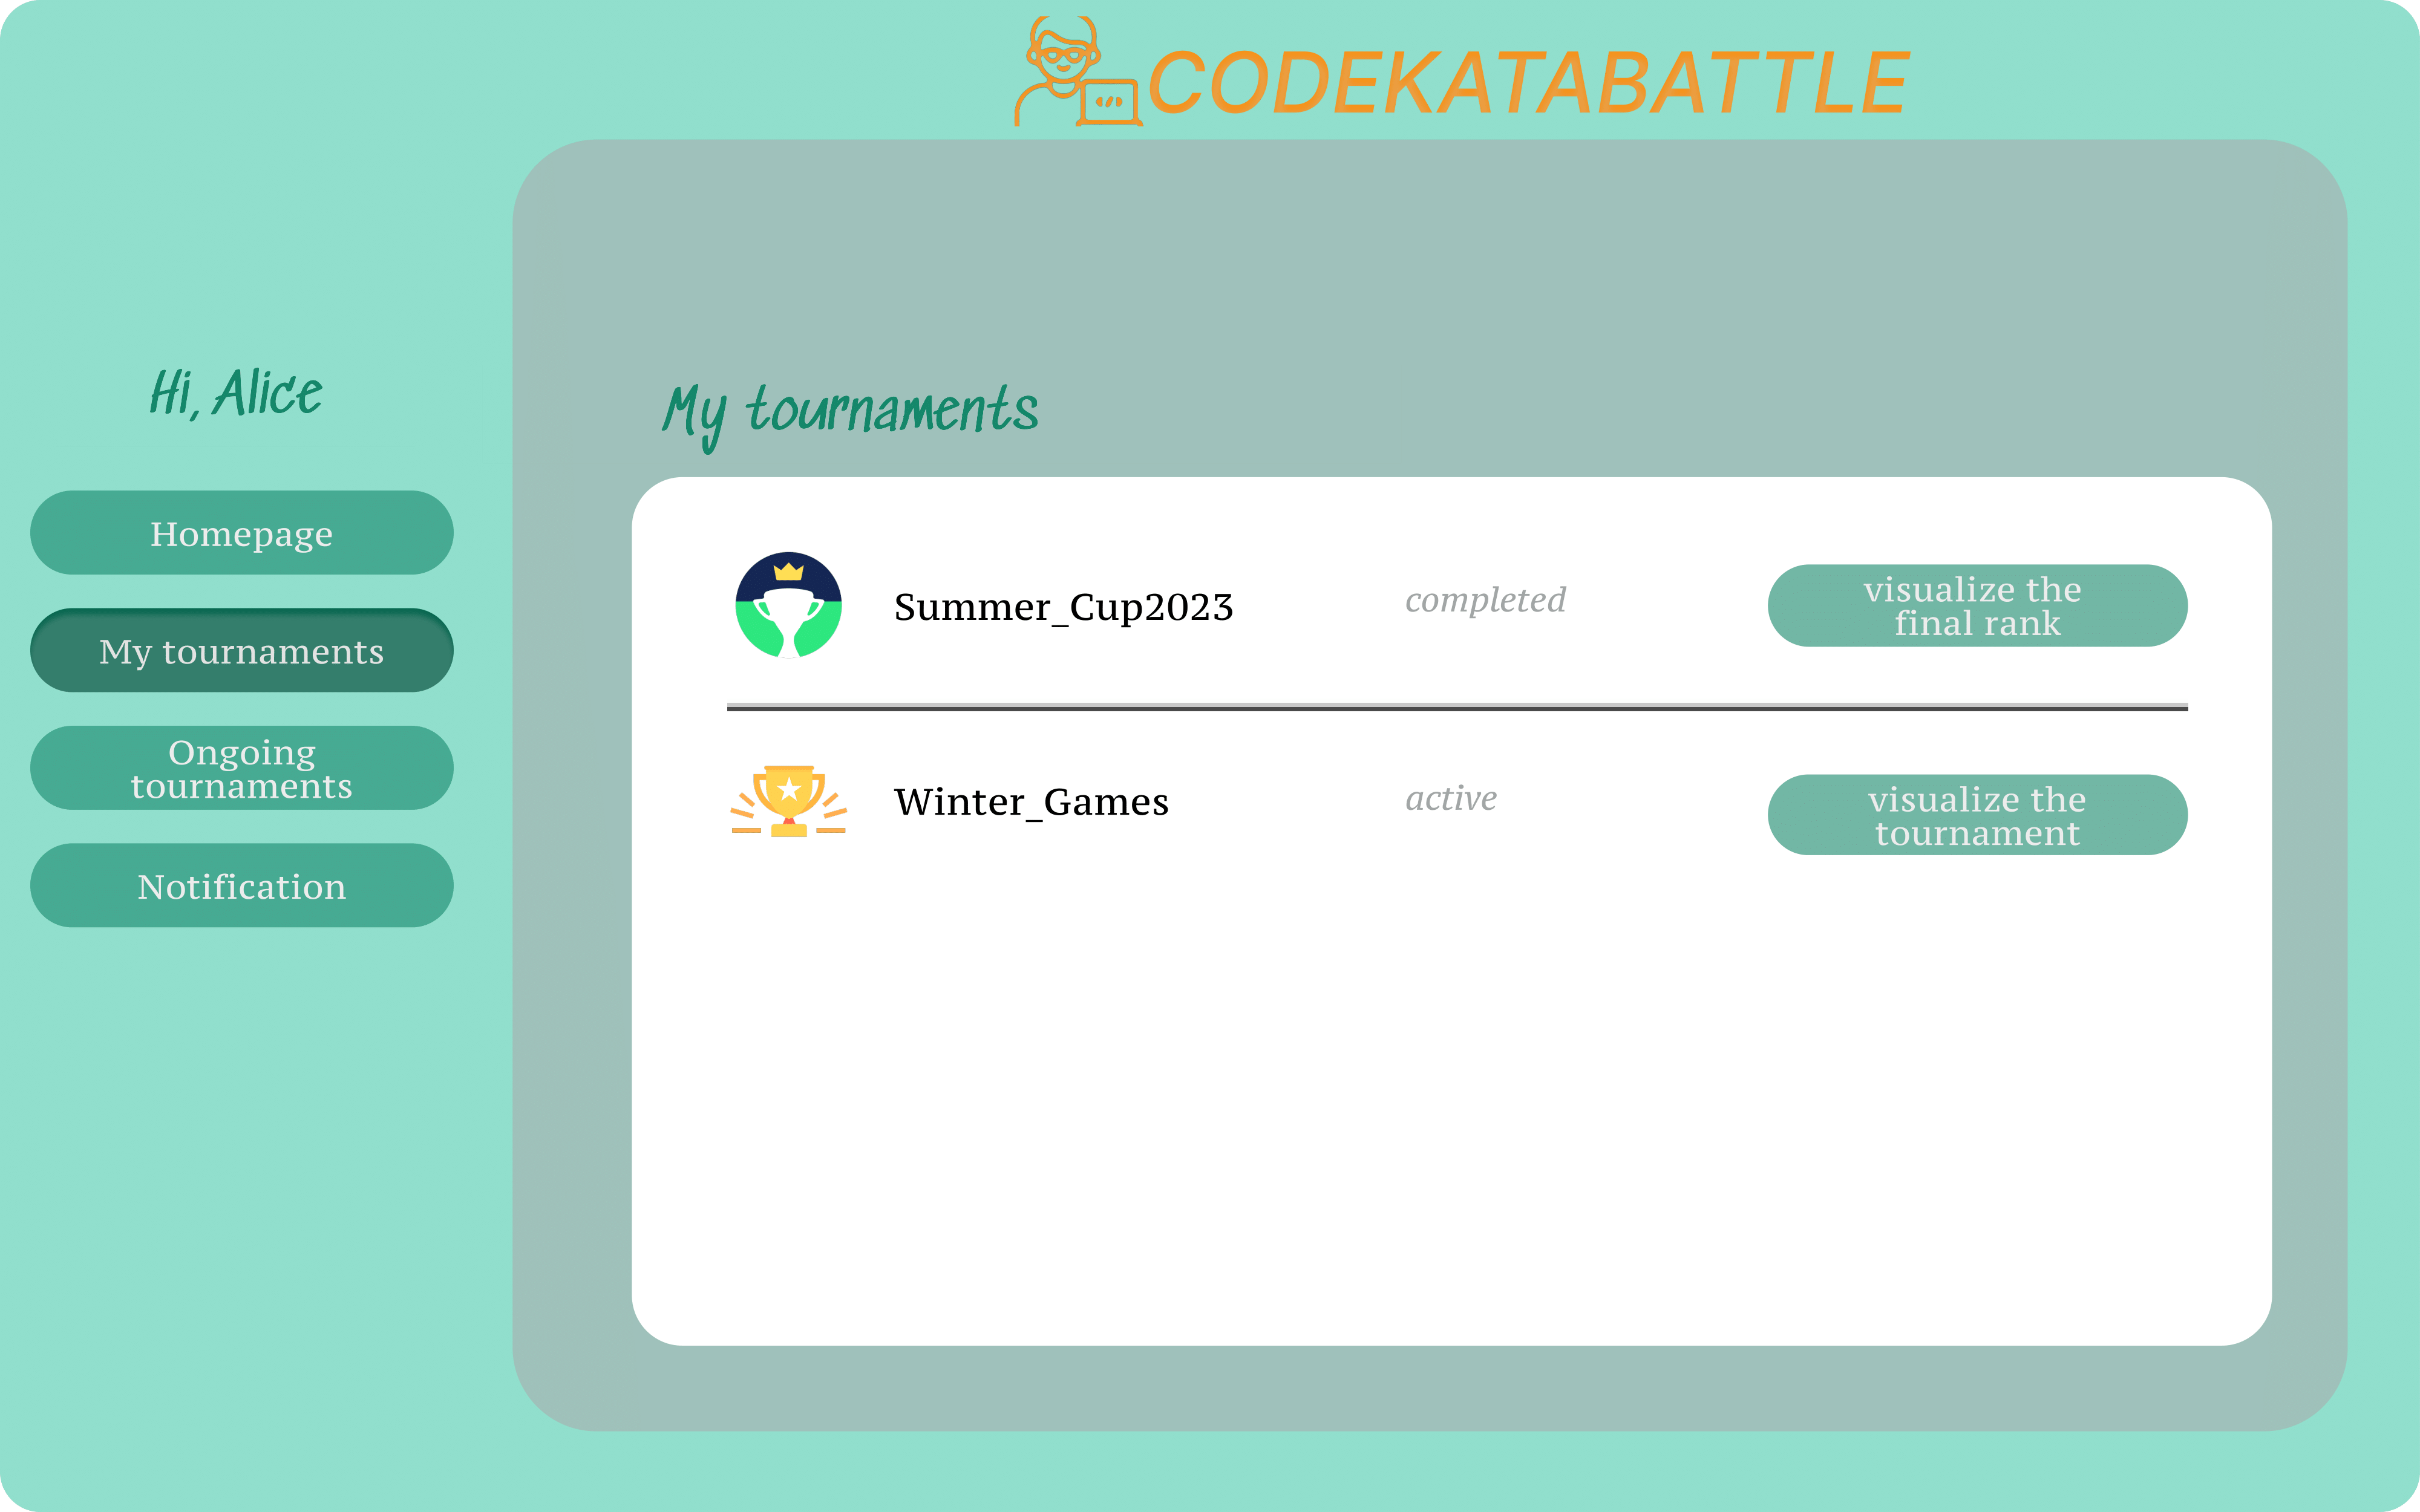
\includegraphics[width=0.8\textwidth]{images/user_interface/UI_sw2-04.png}
    \caption{My tournaments - student's page}
\end{figure}

\begin{figure}[H]
    \centering
    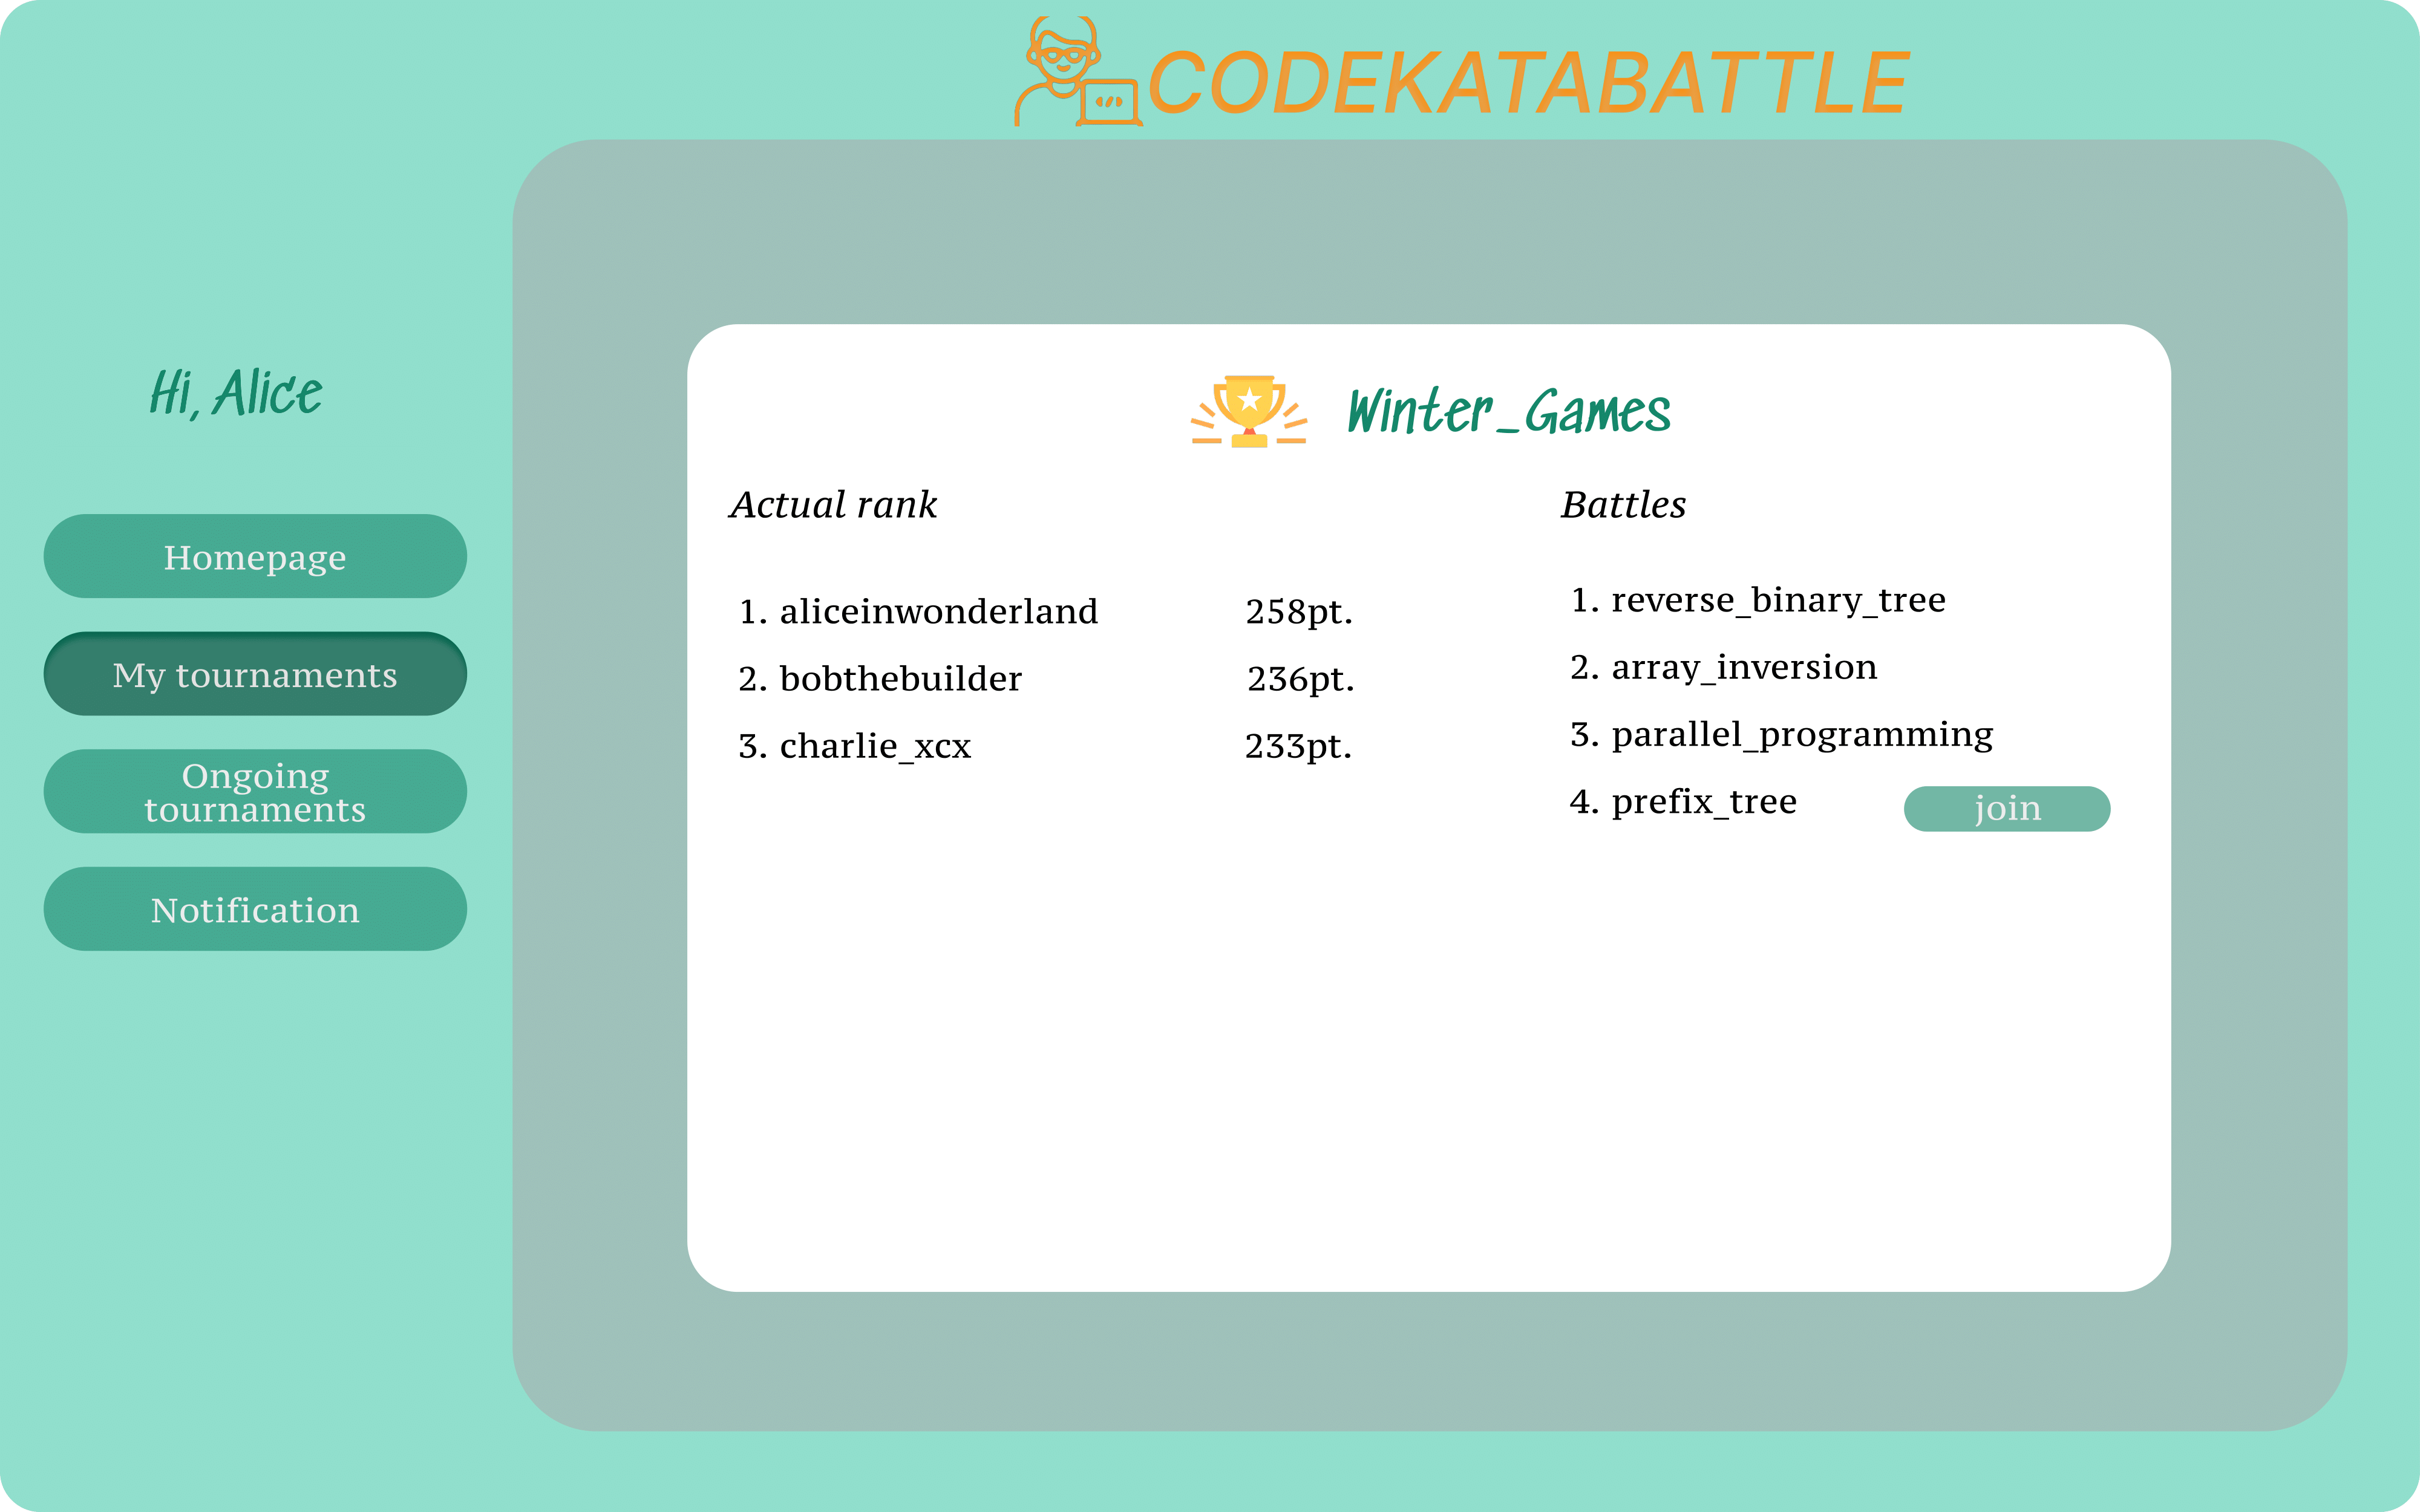
\includegraphics[width=0.8\textwidth]{images/user_interface/UI_sw2-05.png}
    \caption{Tournament's details - student's page}
\end{figure}

\begin{figure}[H]
    \centering
    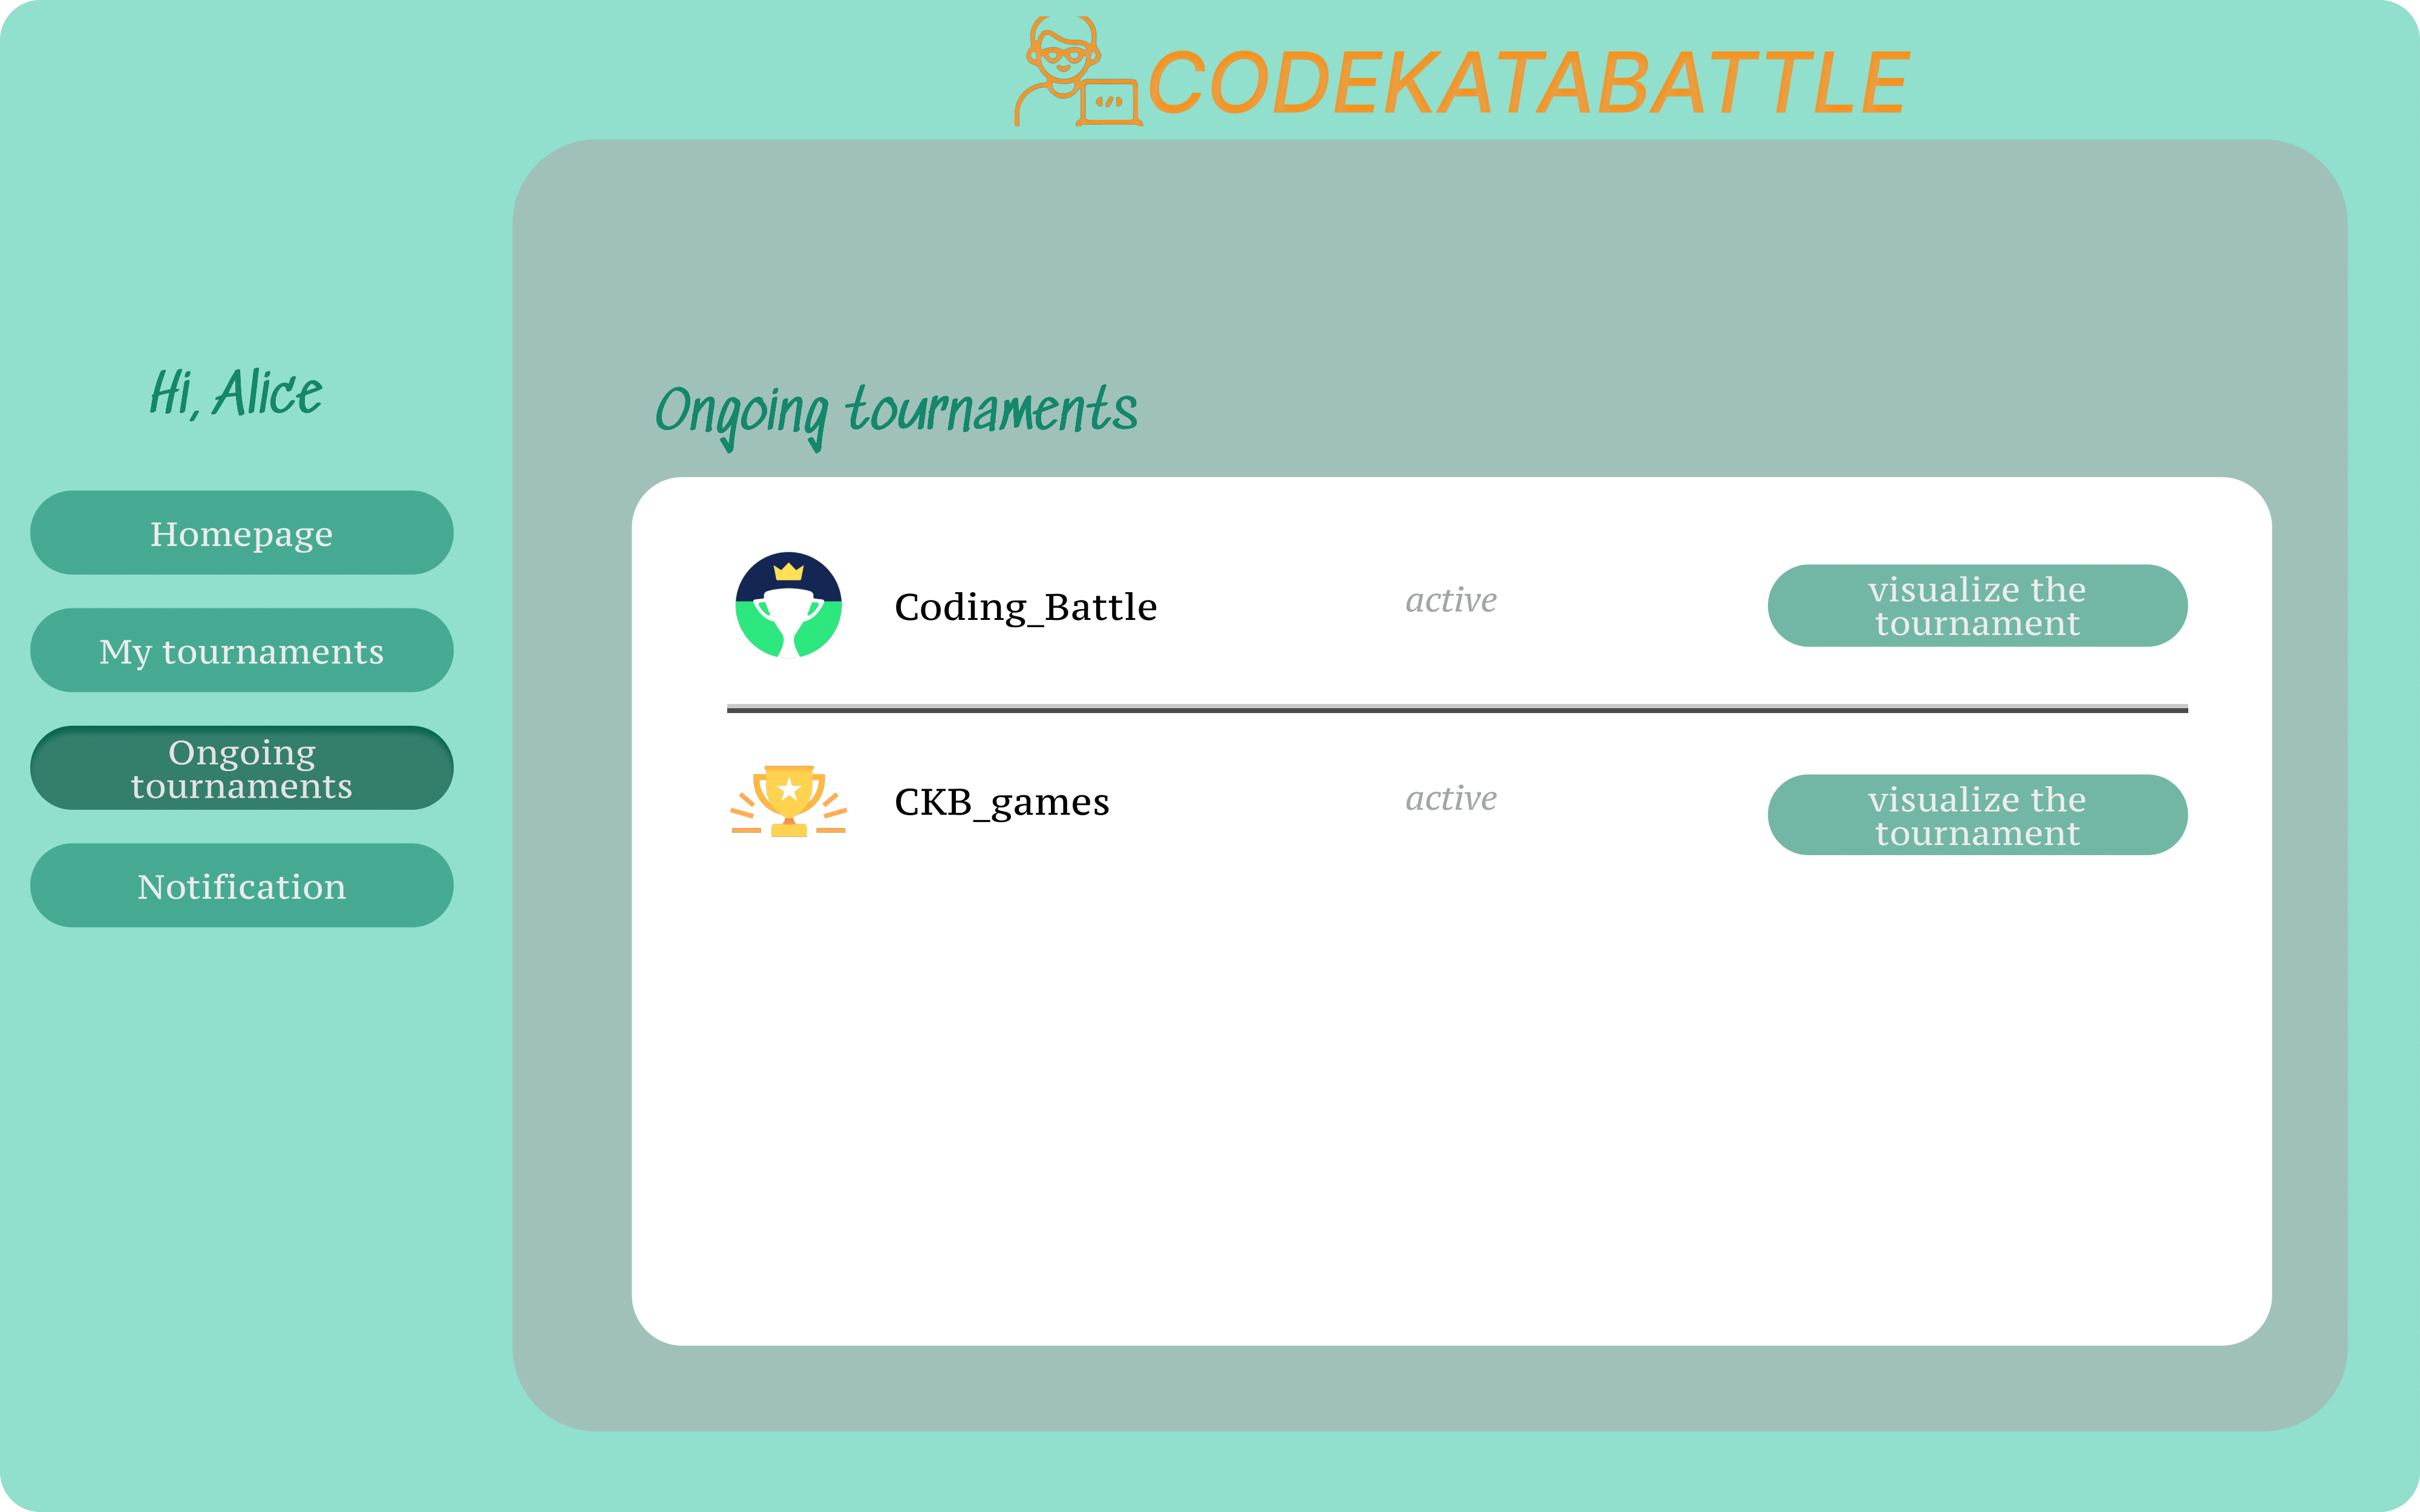
\includegraphics[width=0.8\textwidth]{images/user_interface/UI_sw2-06.png}
    \caption{Ongoing tournaments - student's page}
\end{figure}

\begin{figure}[H]
    \centering
    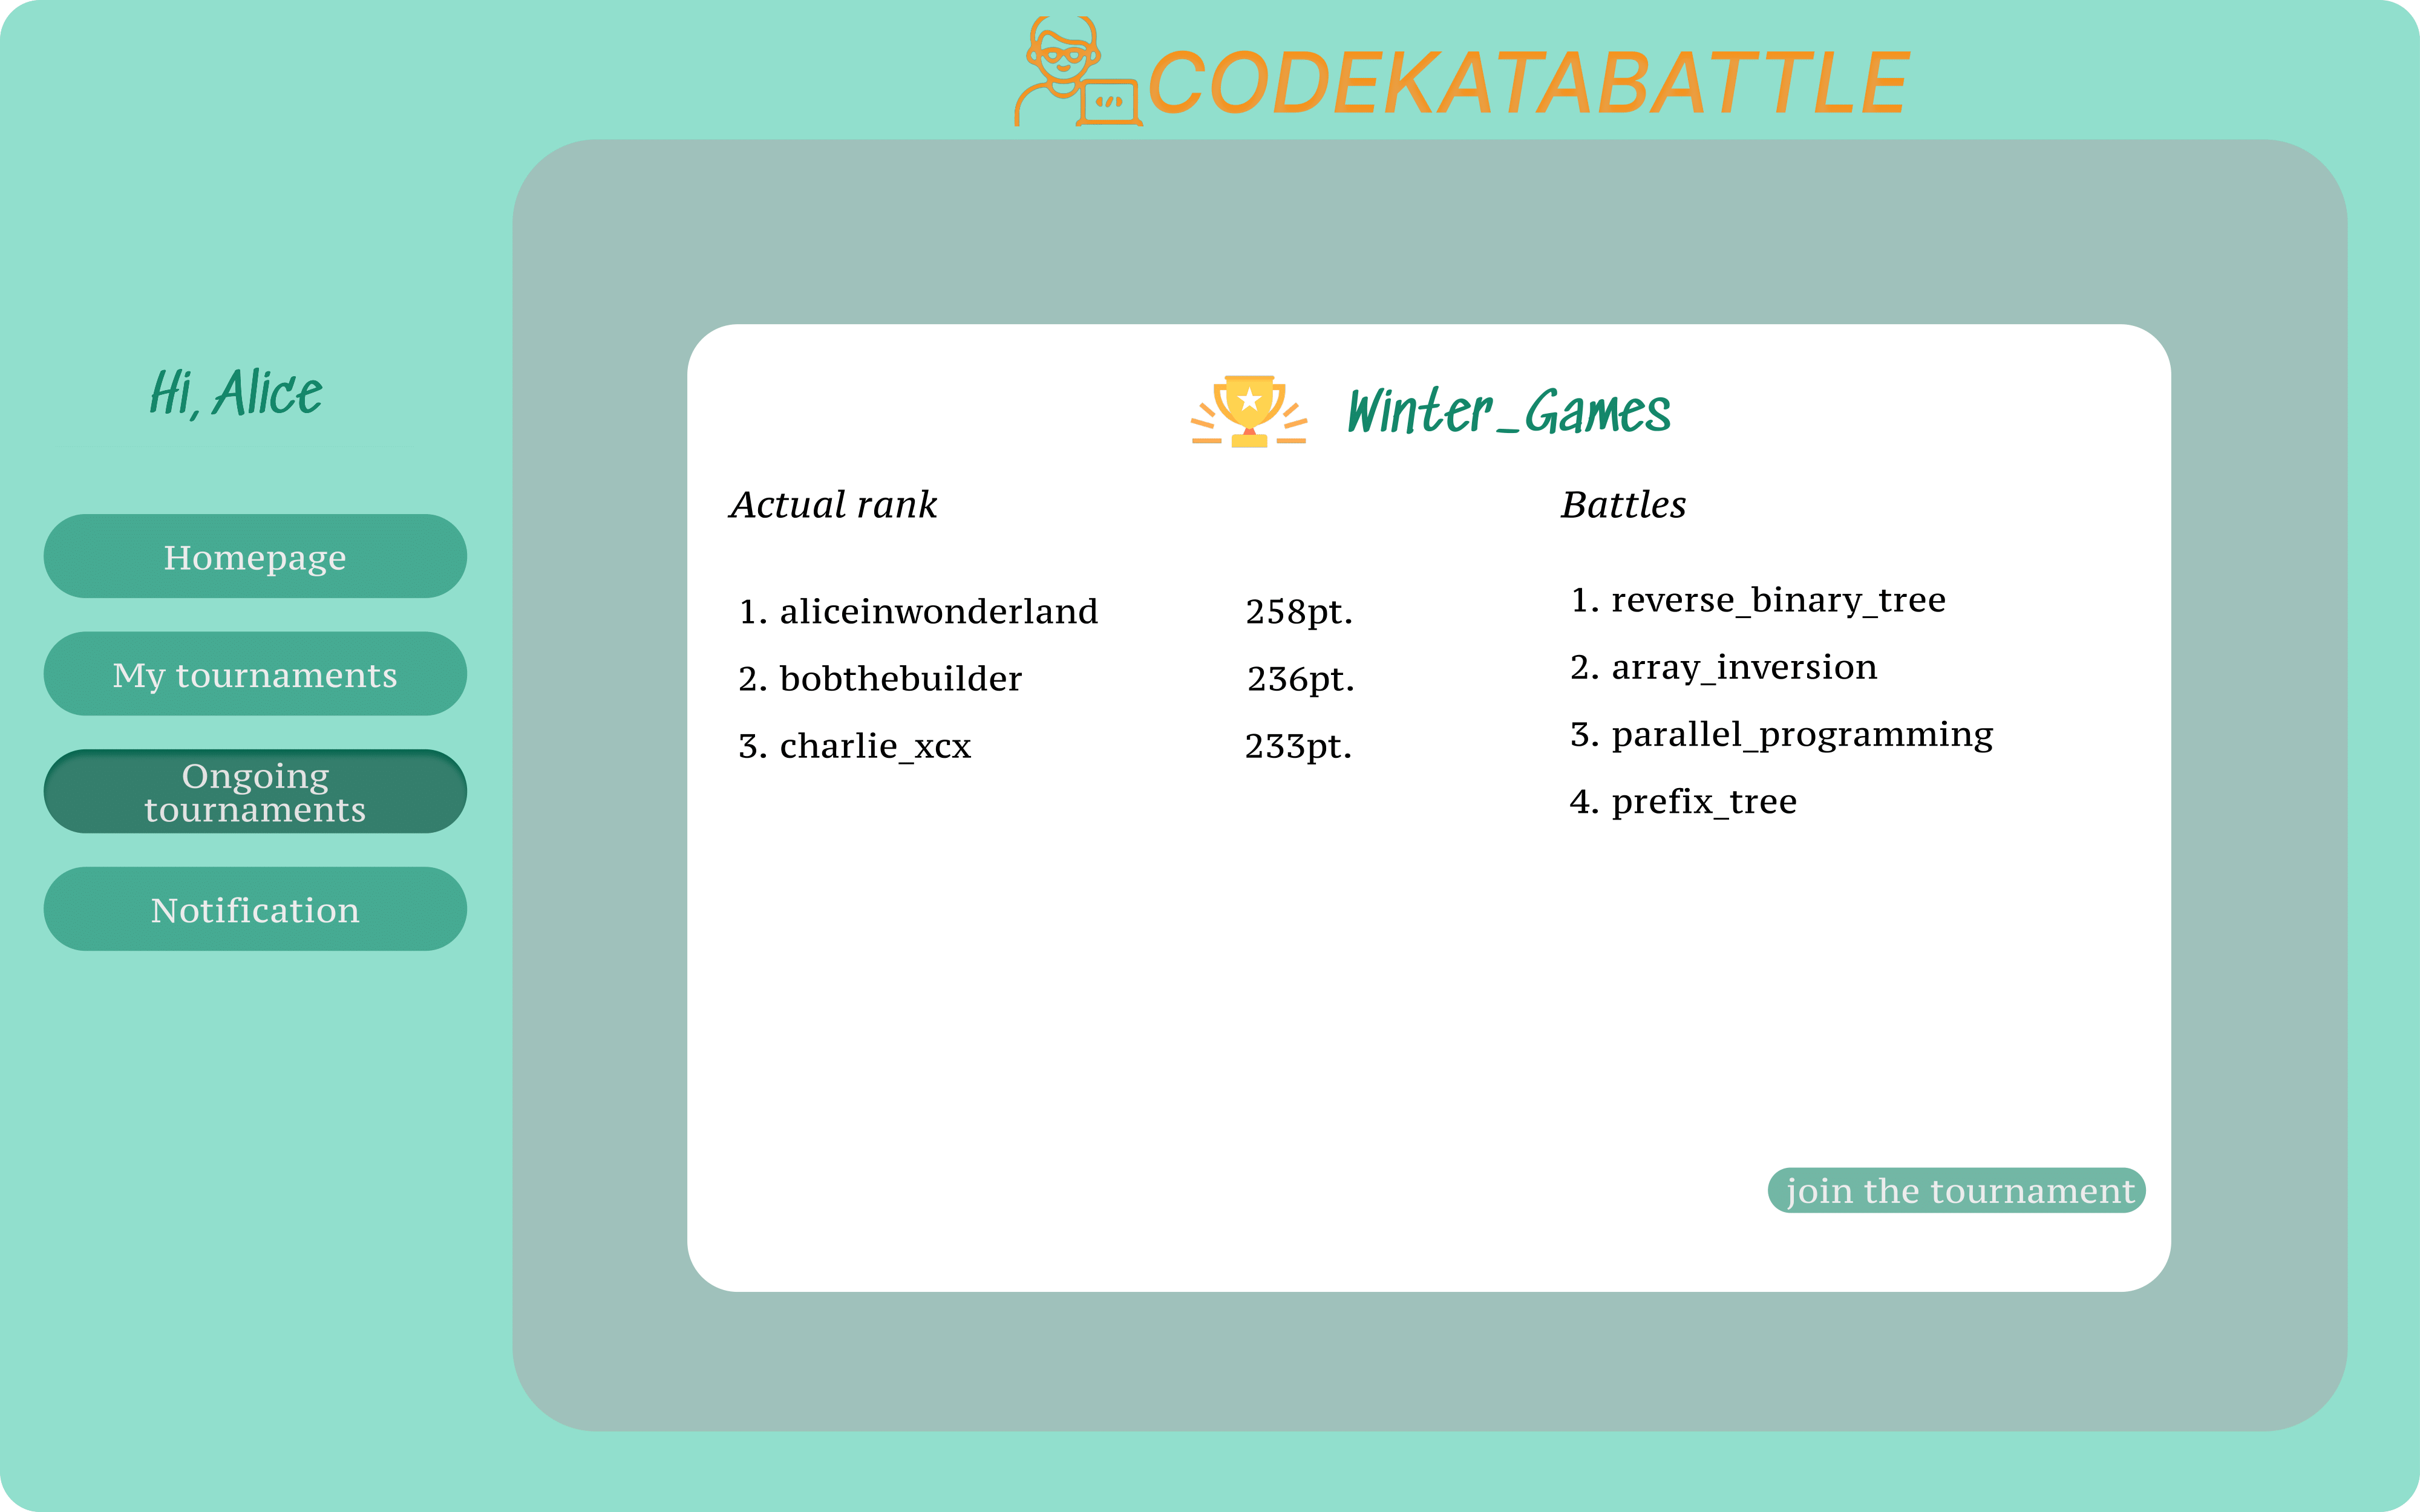
\includegraphics[width=0.8\textwidth]{images/user_interface/UI_sw2-07.png}
    \caption{Join a new tournament - student's page}
\end{figure}

\begin{figure}[H]
    \centering
    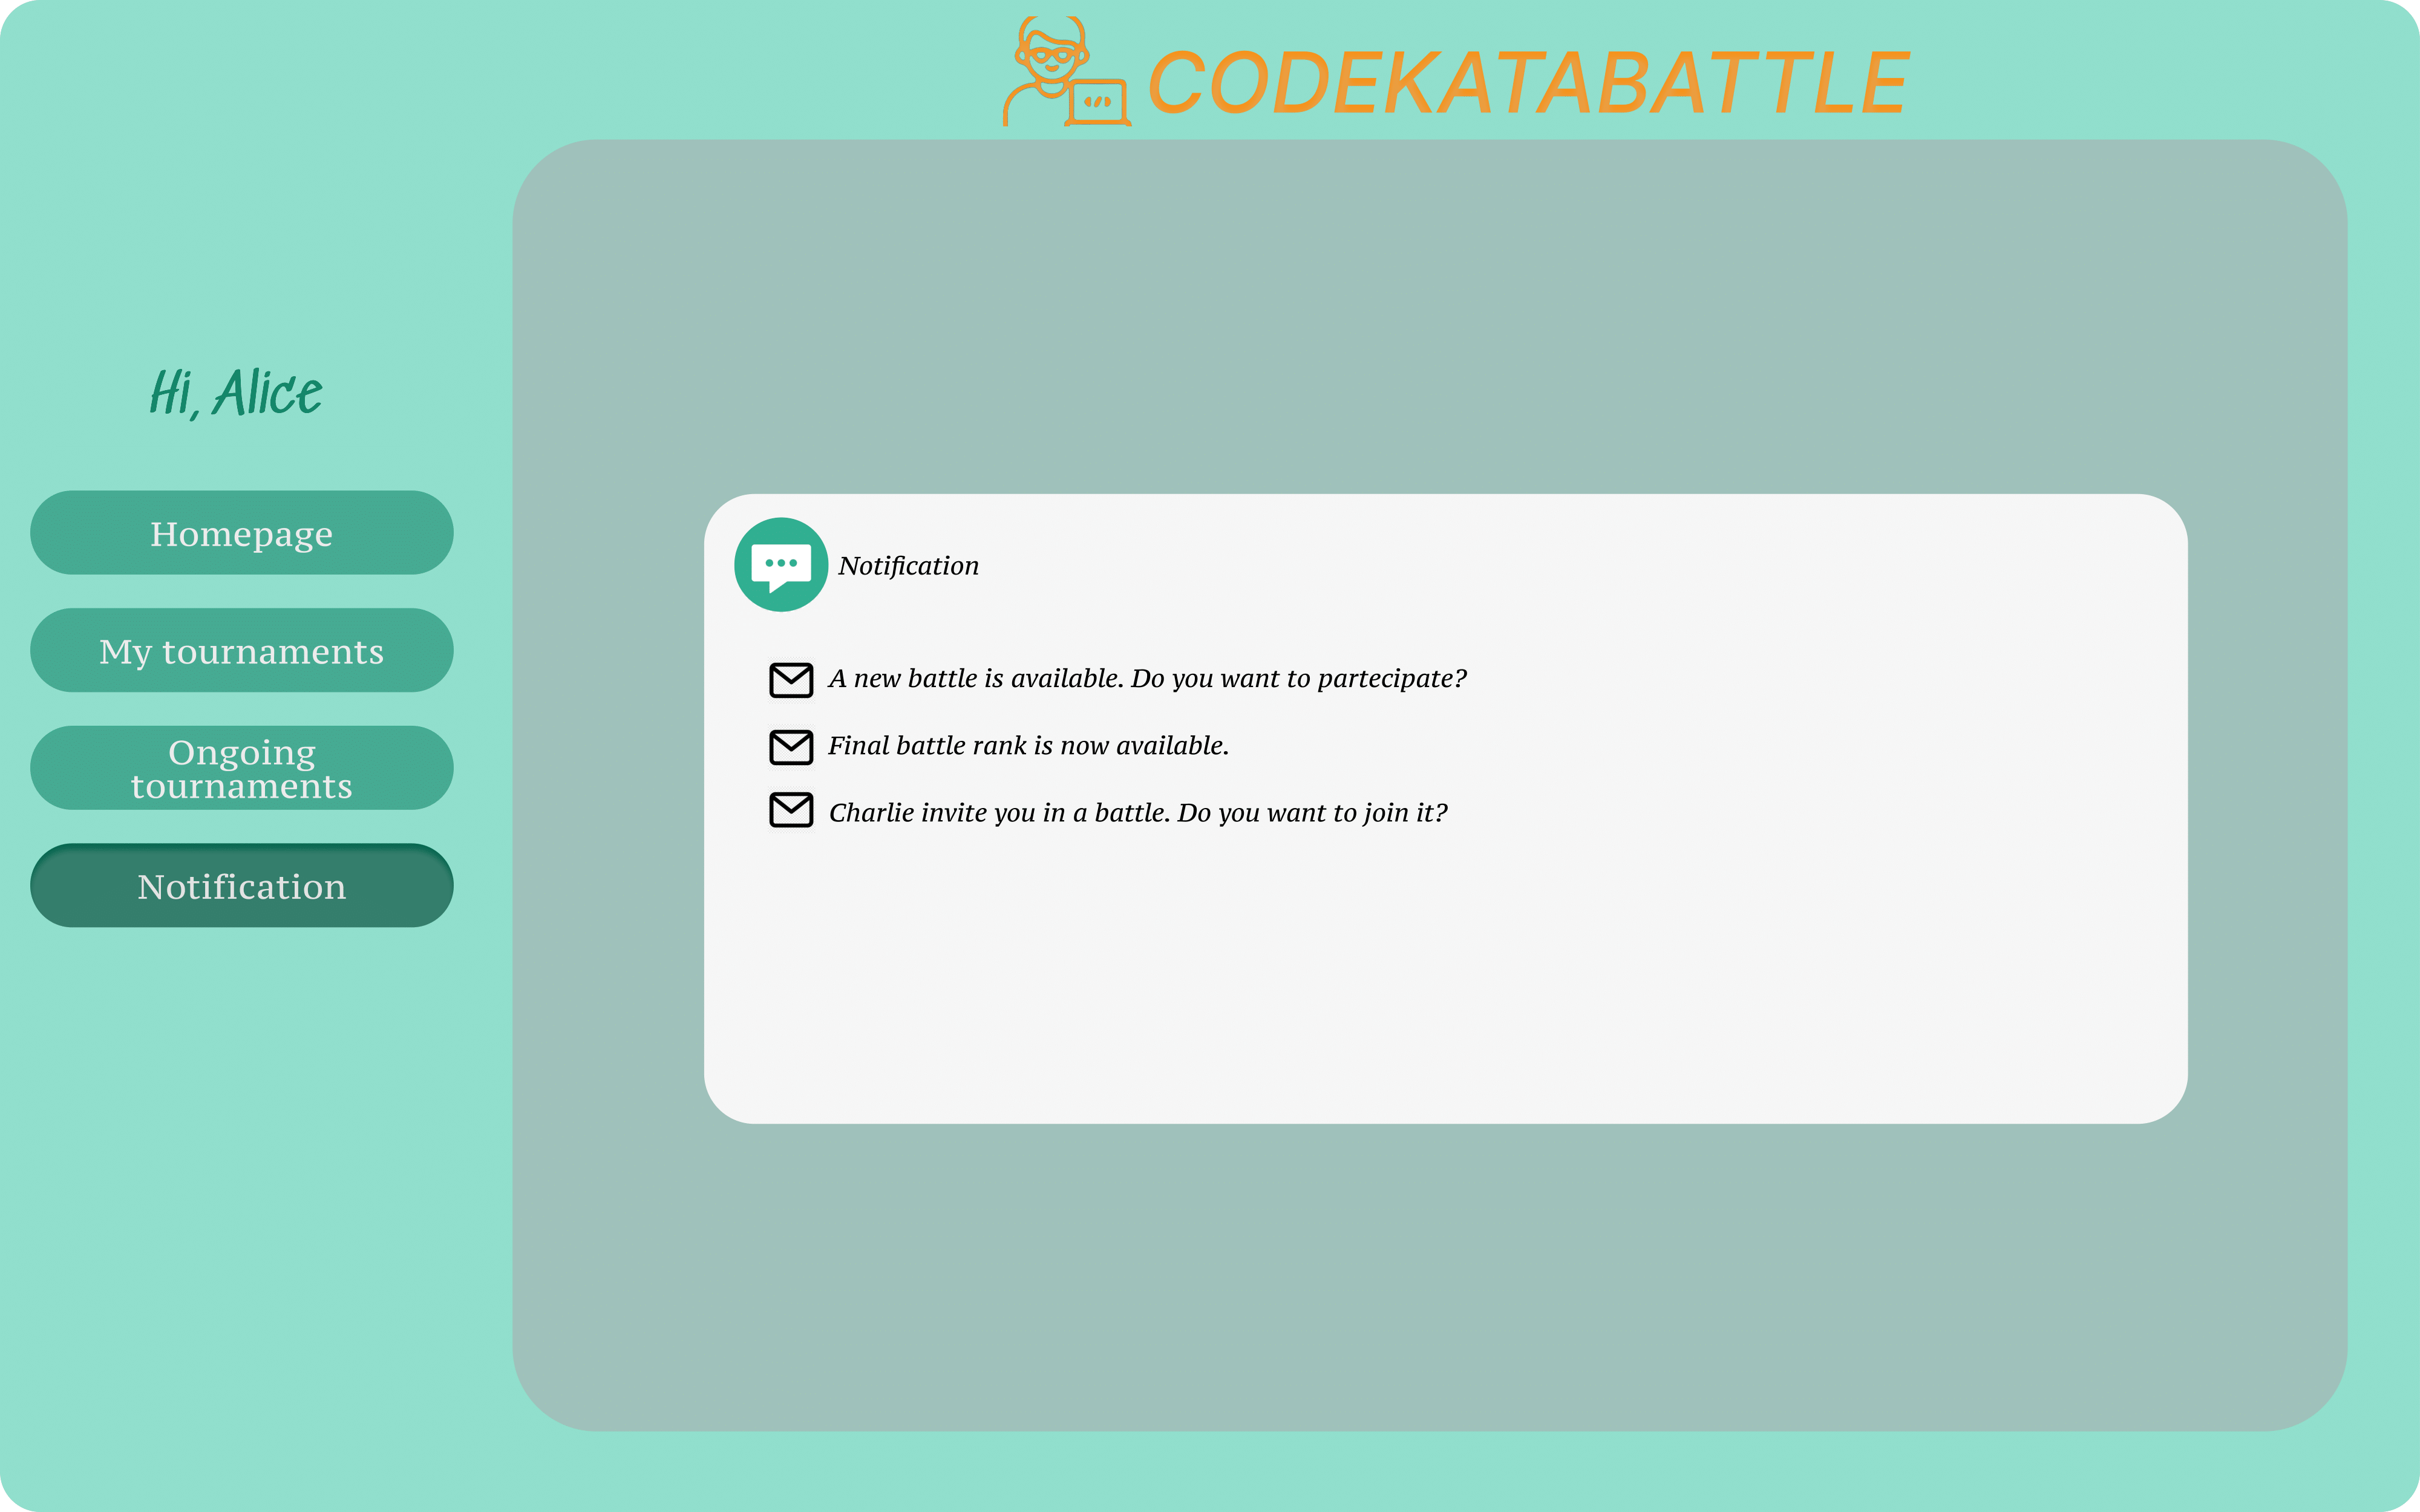
\includegraphics[width=0.8\textwidth]{images/user_interface/UI_sw2-08.png}
    \caption{Notification page - student's page}
\end{figure}

\begin{figure}[H]
    \centering
    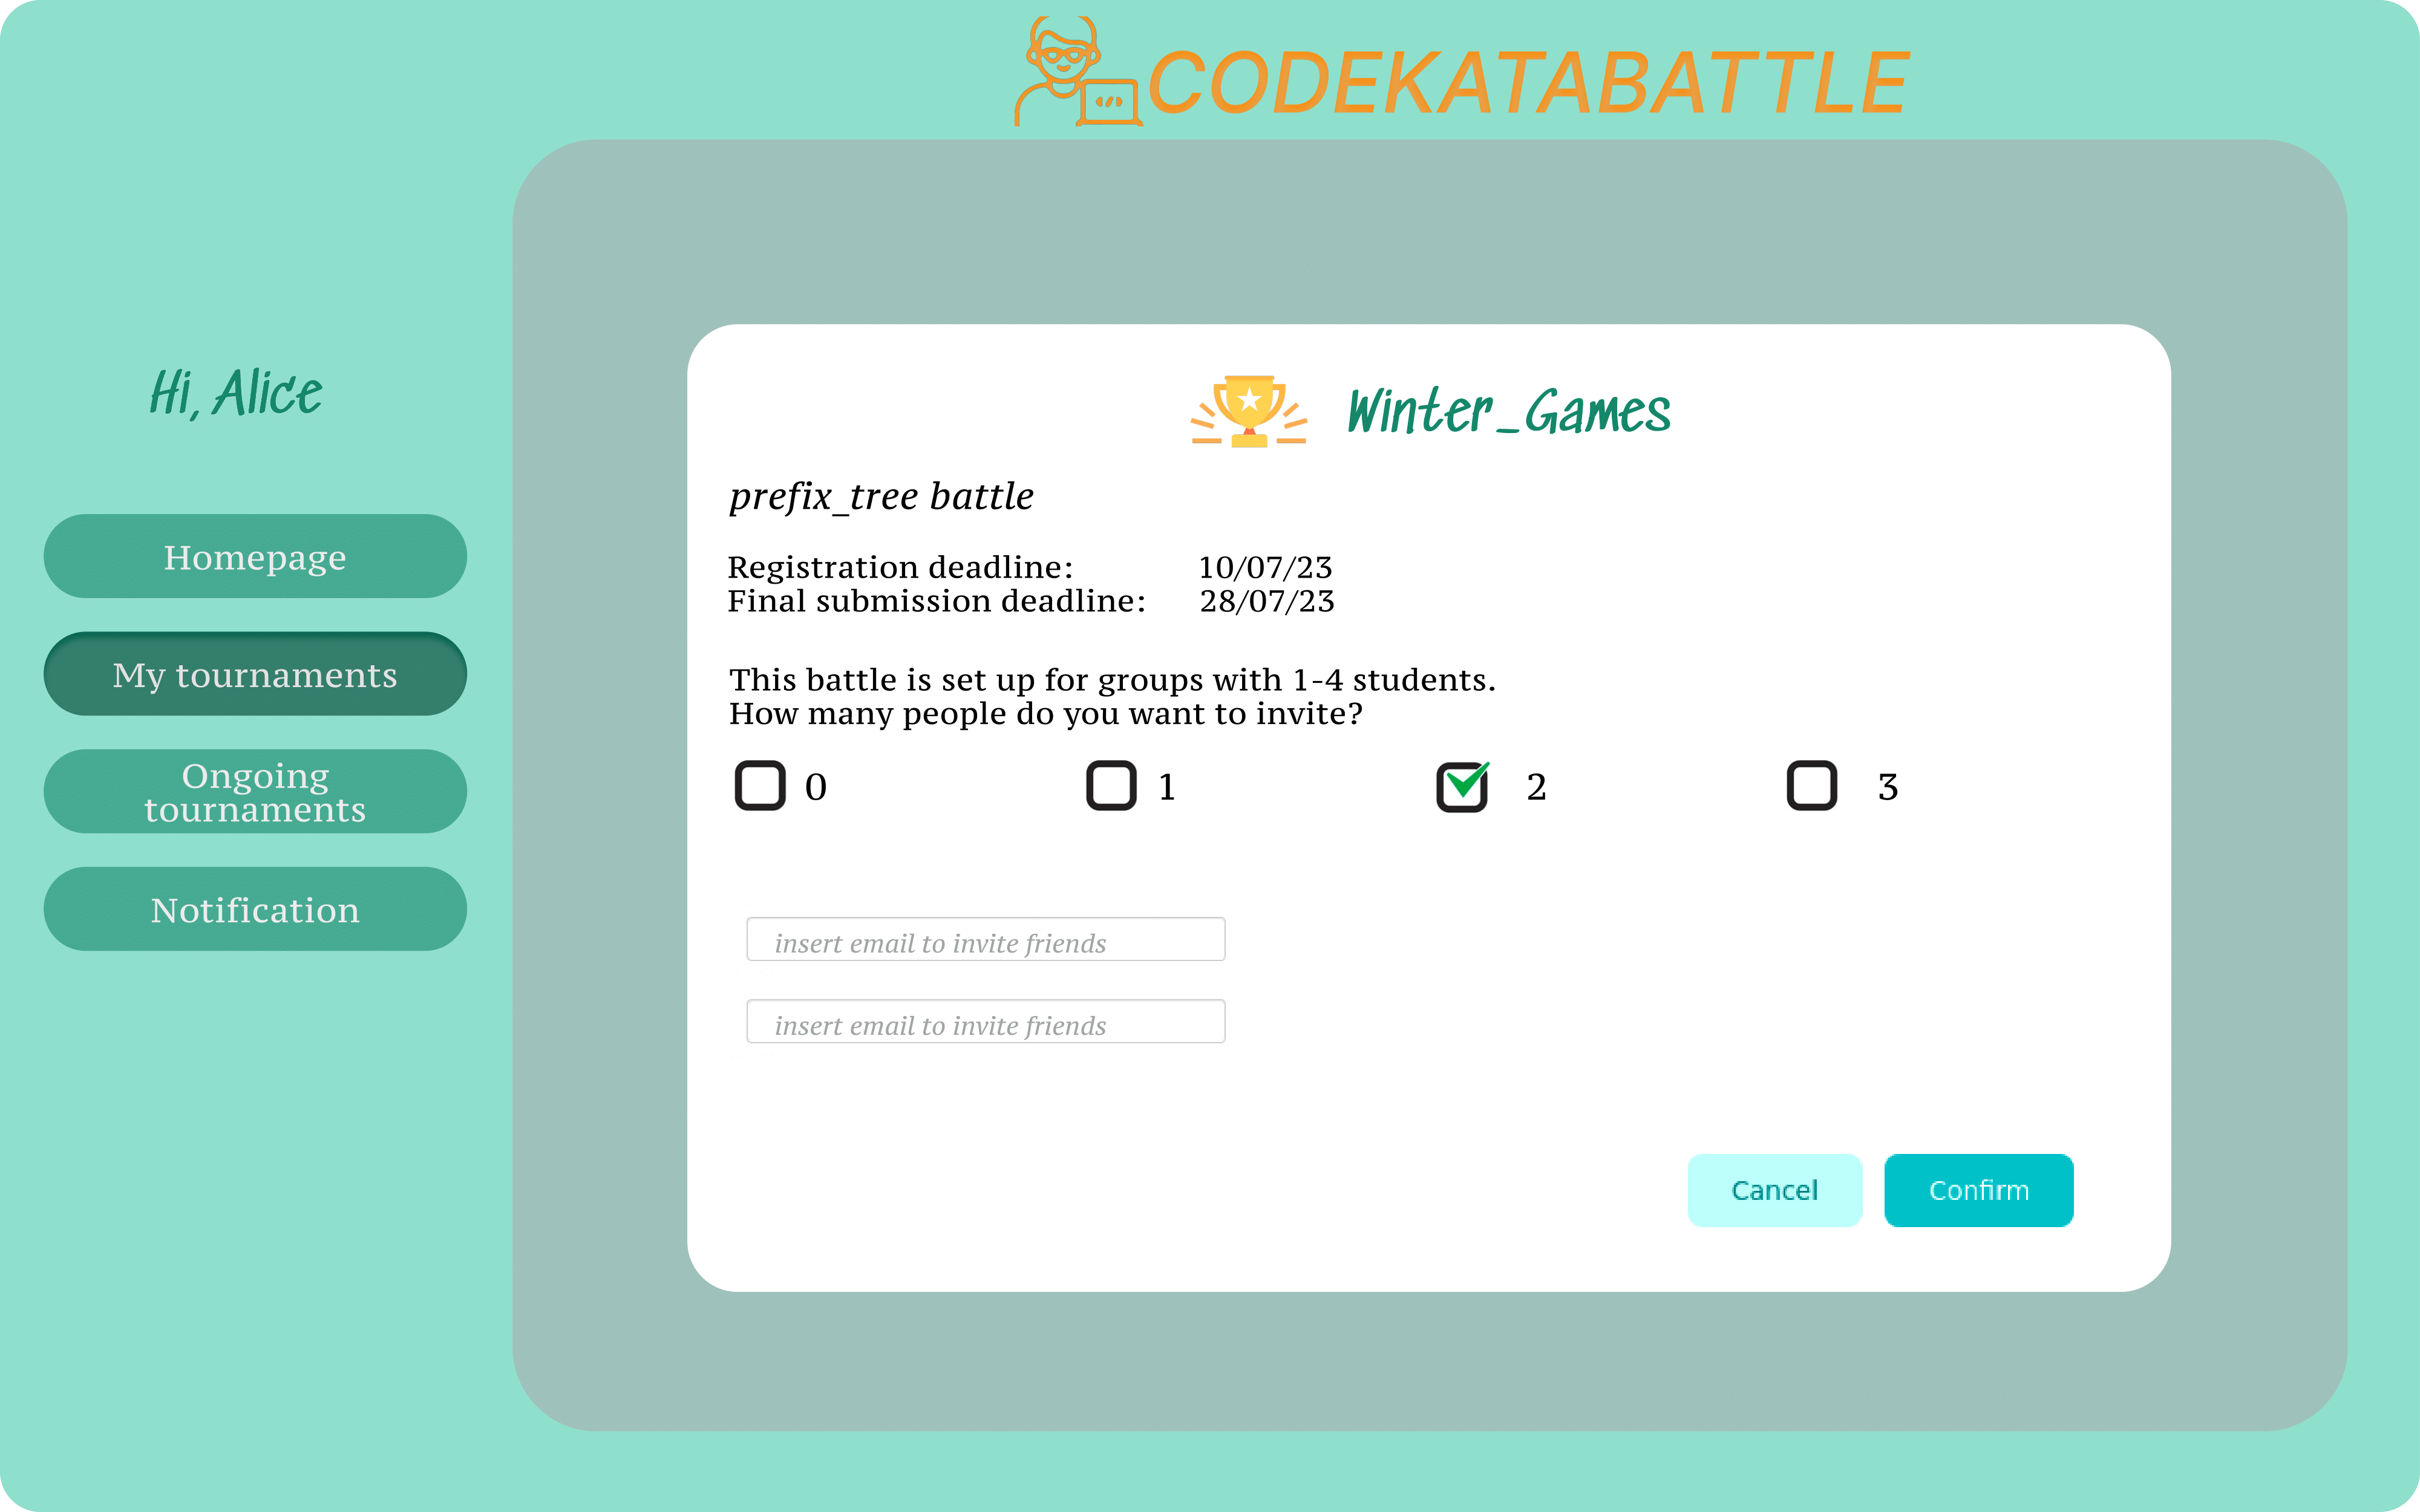
\includegraphics[width=0.8\textwidth]{images/user_interface/UI_sw2-09.png}
    \caption{Submission of a new battle - student's page}
\end{figure}

\begin{figure}[H]
    \centering
    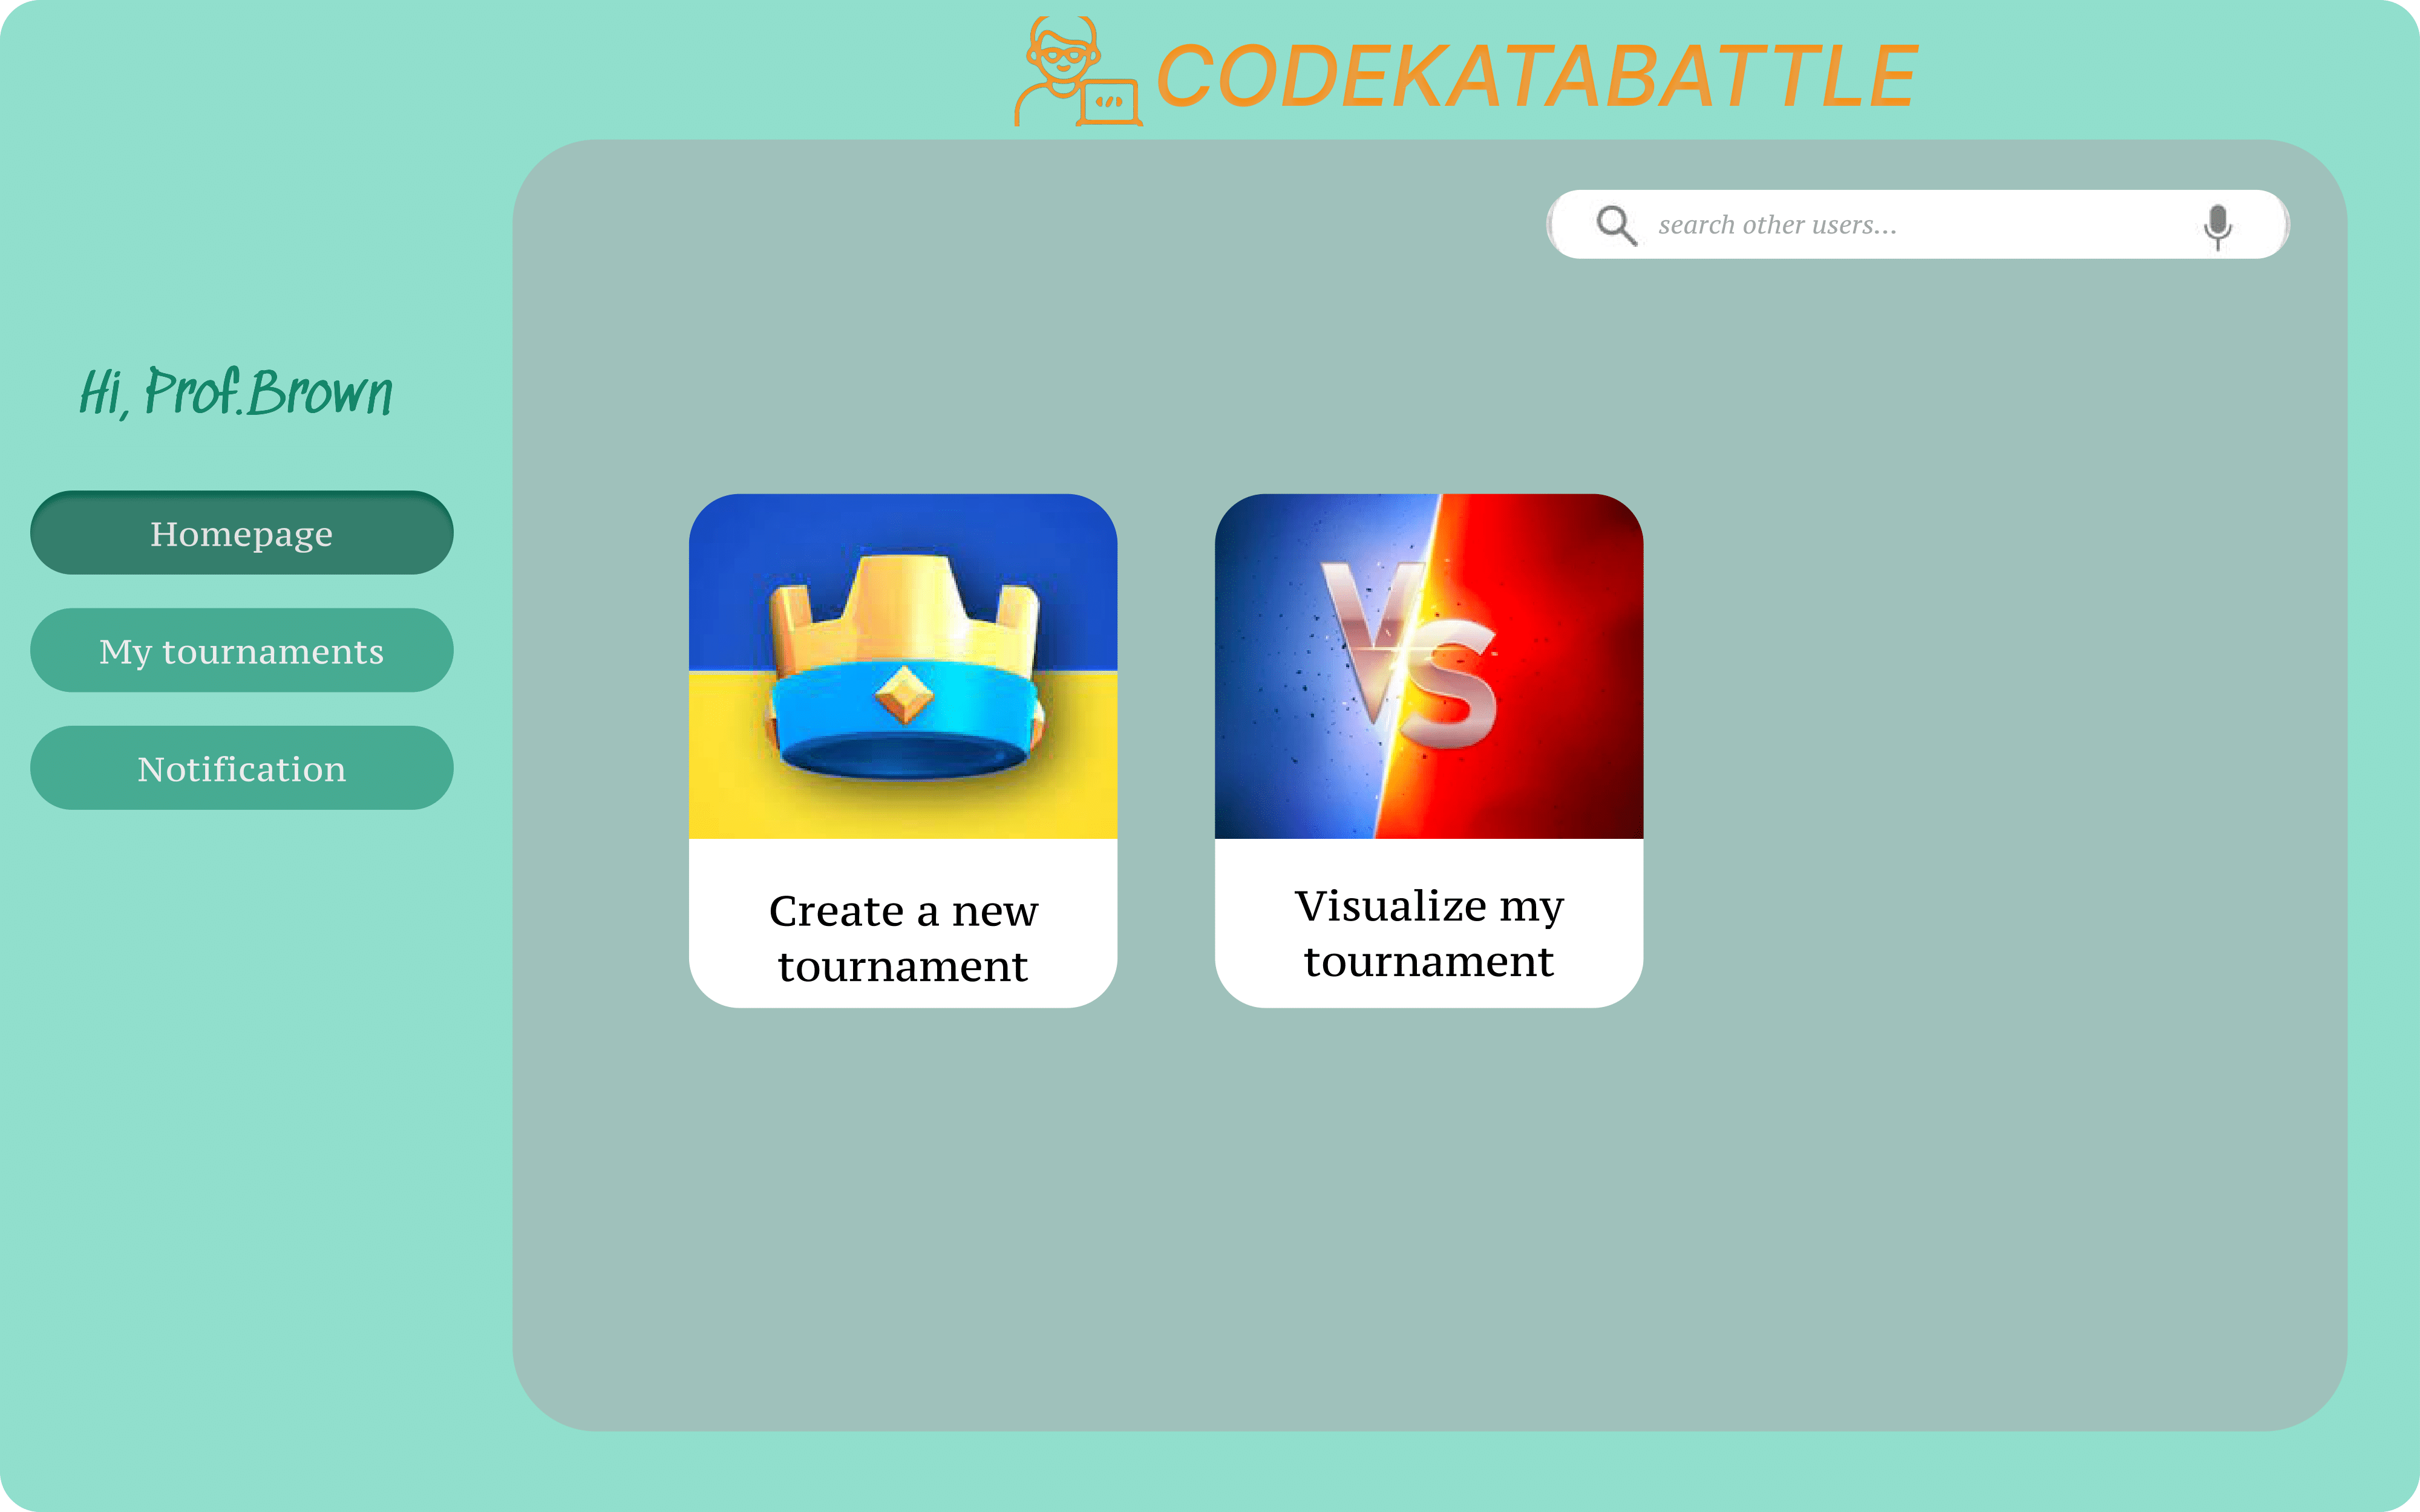
\includegraphics[width=0.8\textwidth]{images/user_interface/UI_sw2-10.png}
    \caption{Educator's homepage}
\end{figure}

\begin{figure}[H]
    \centering
    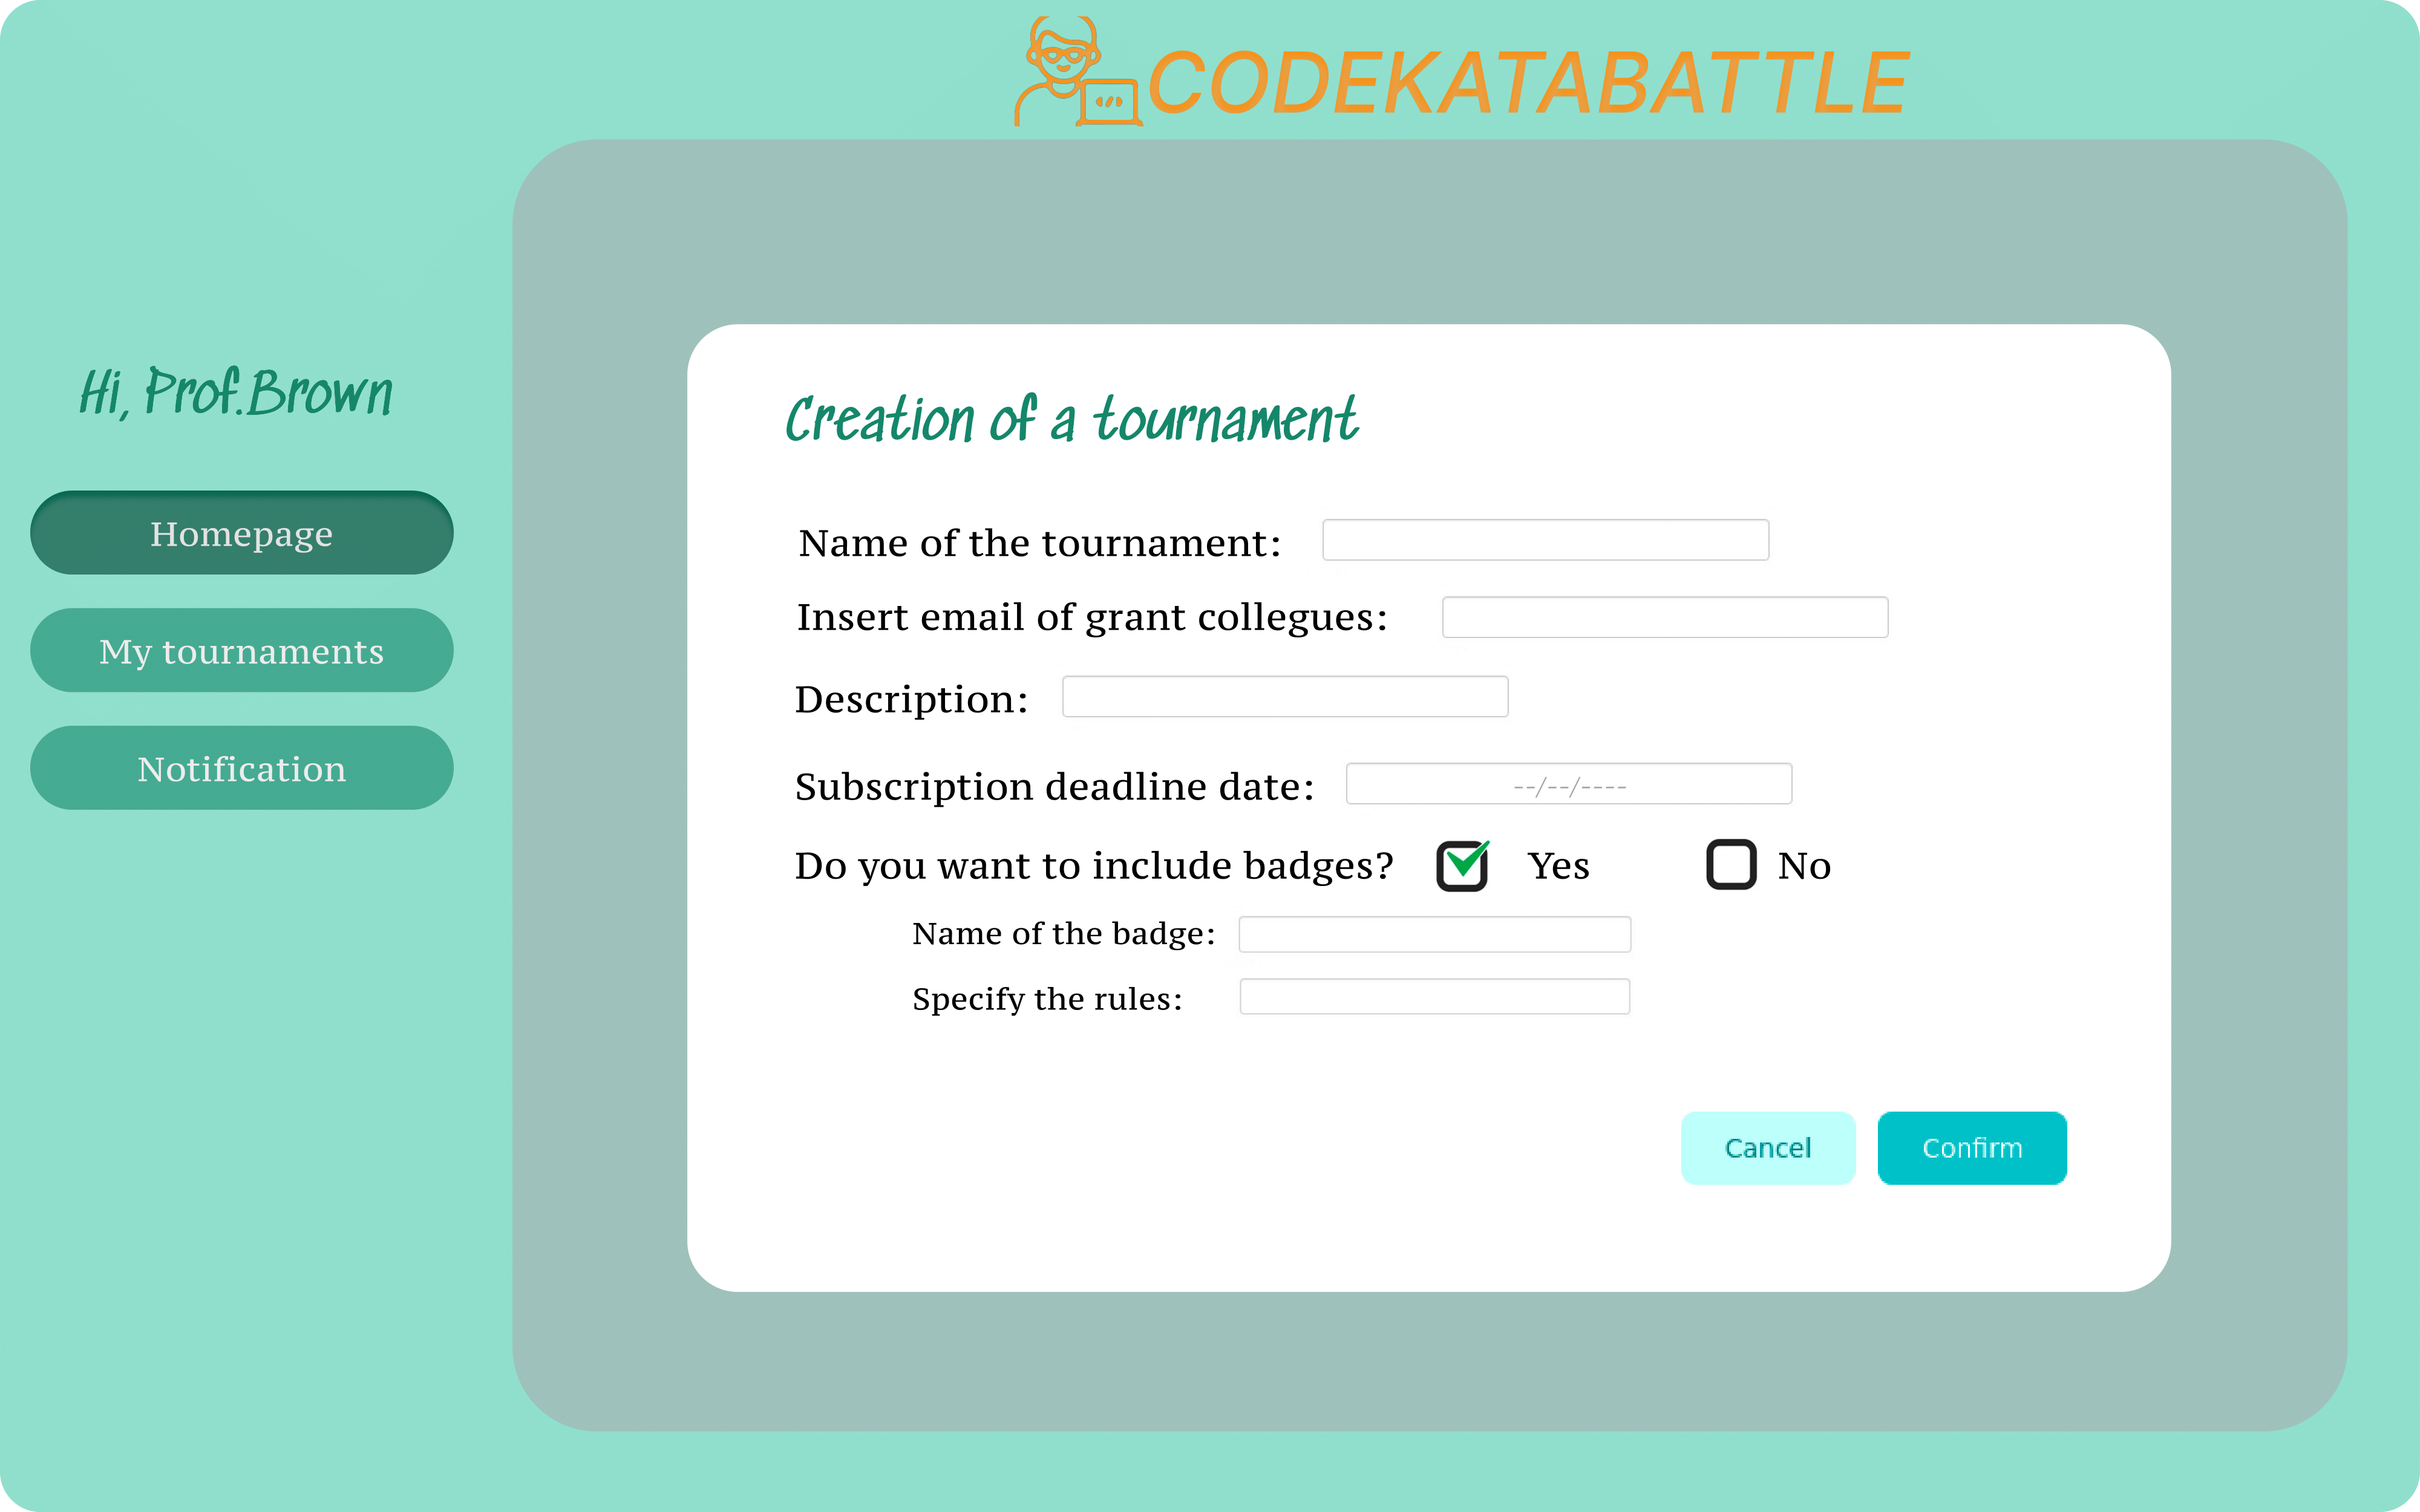
\includegraphics[width=0.8\textwidth]{images/user_interface/UI_sw2-11.png}
    \caption{Creation of a tournament page - educator's page}
\end{figure}

\begin{figure}[H]
    \centering
    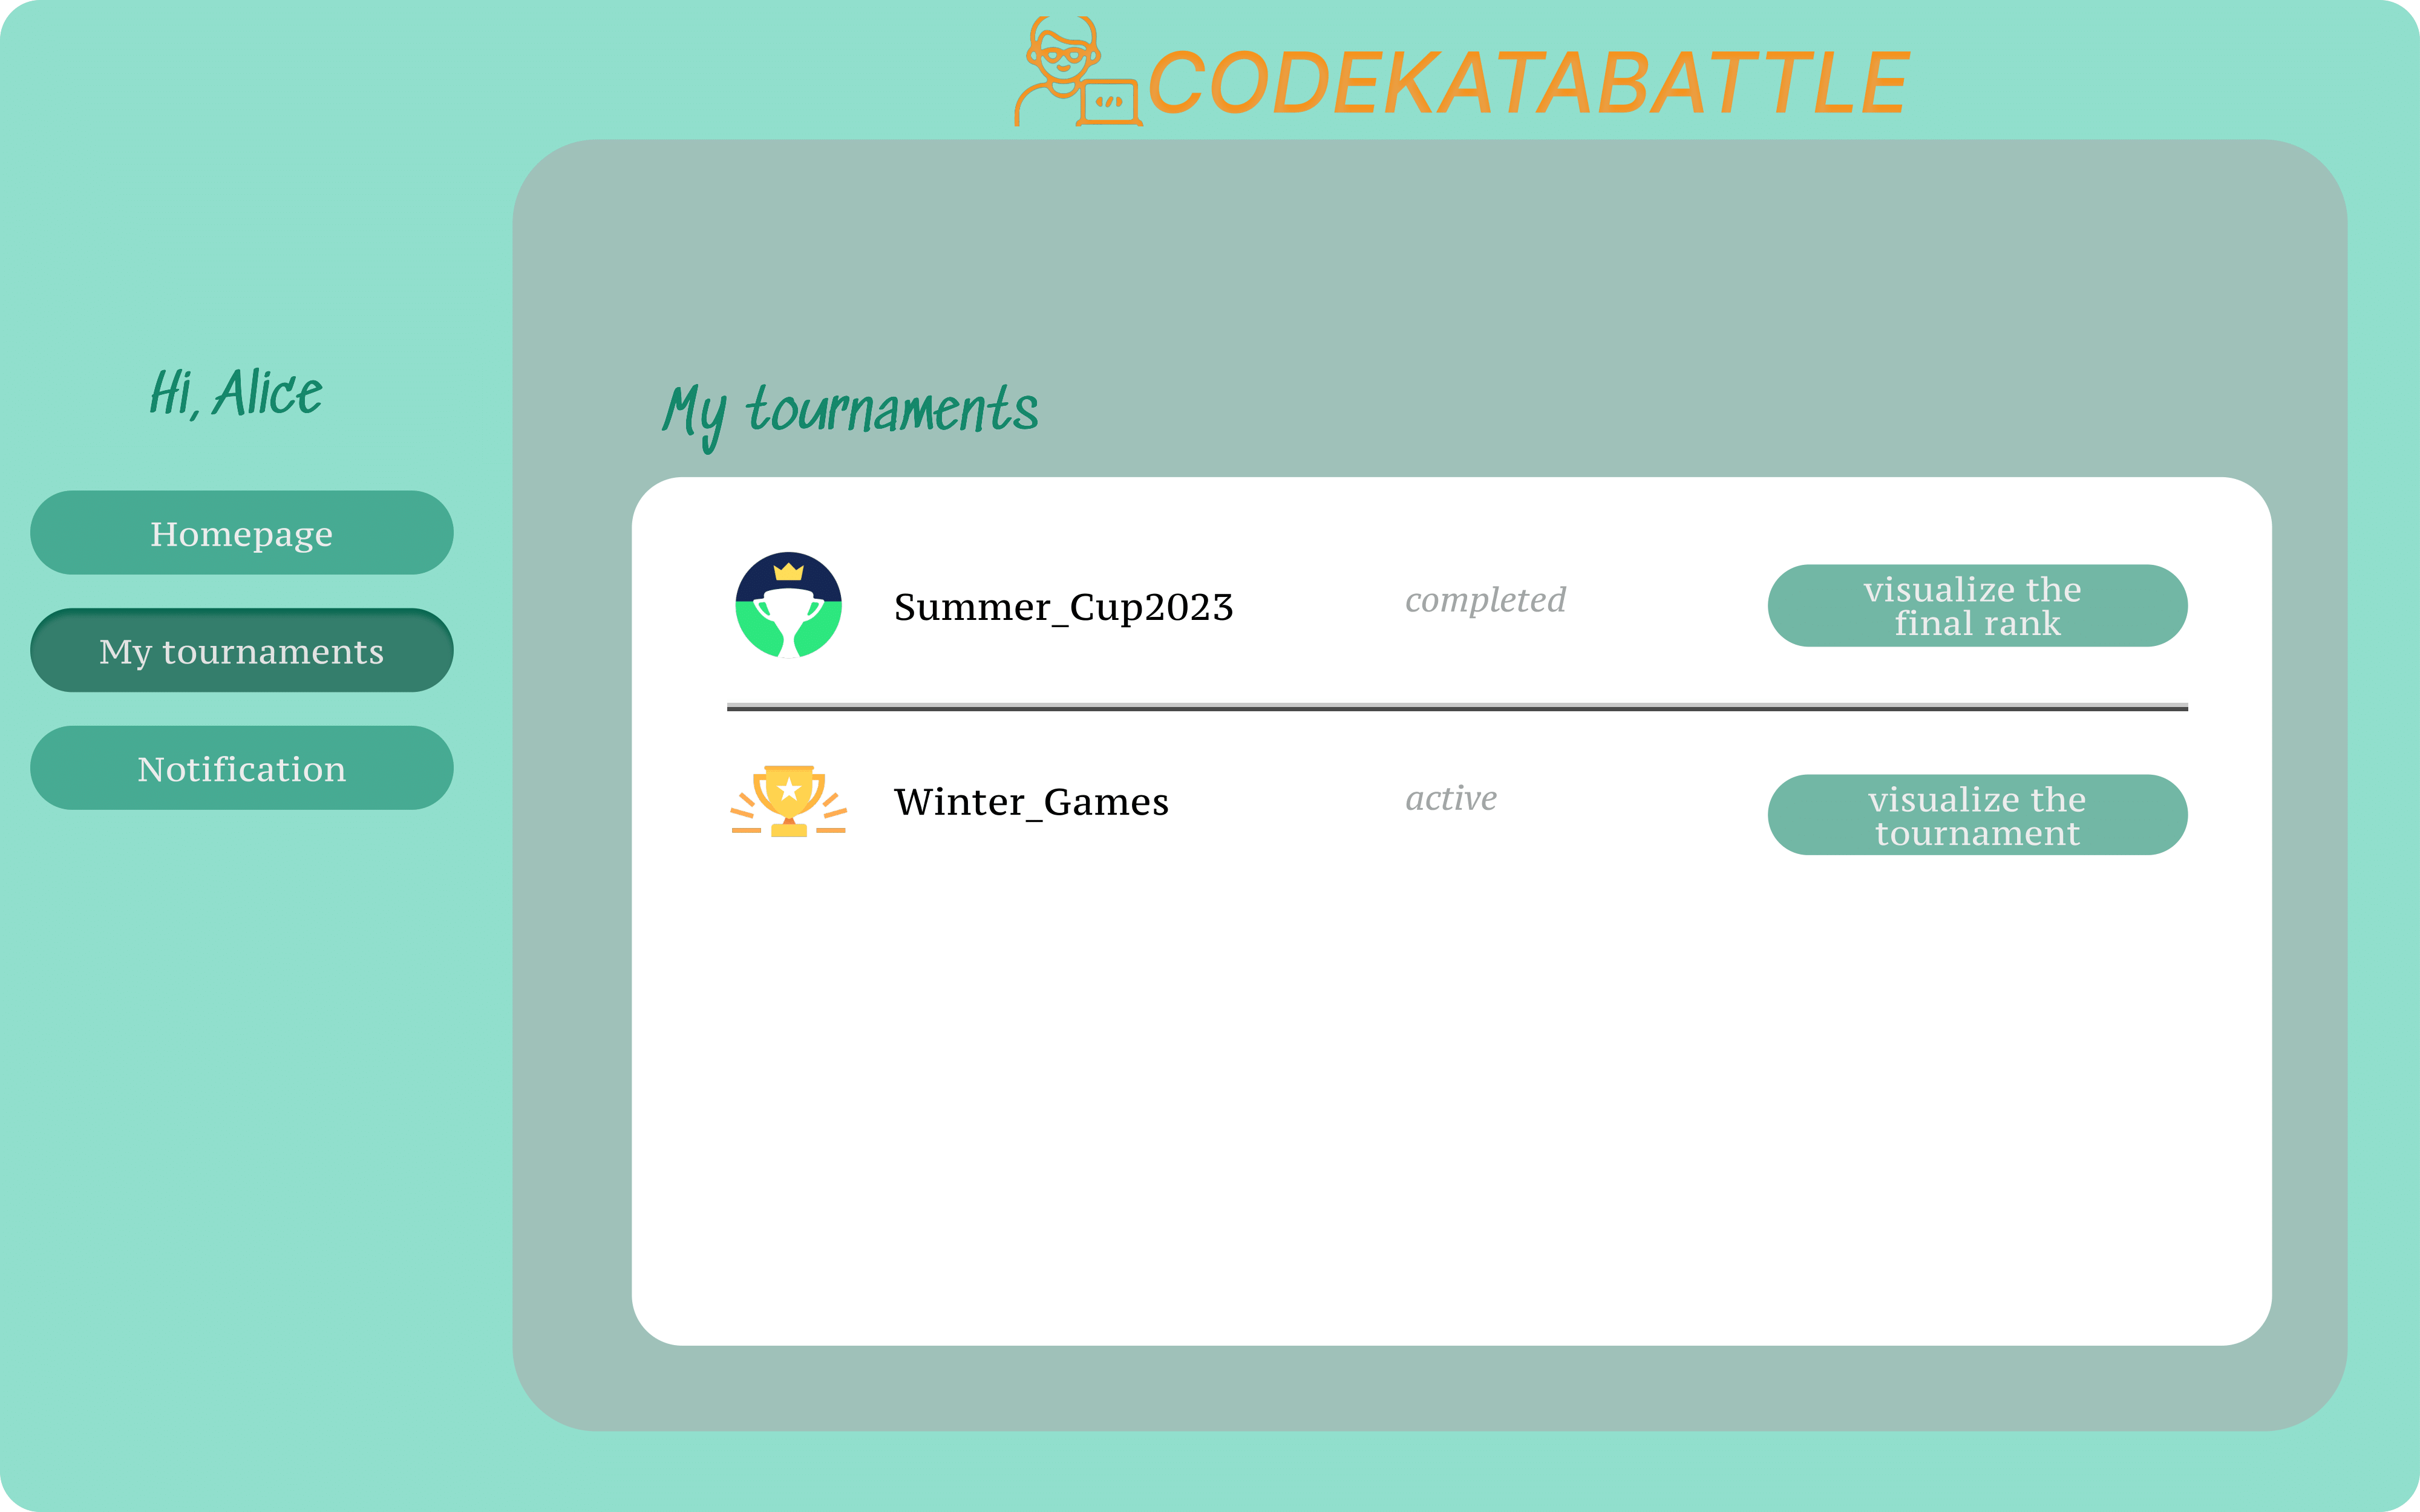
\includegraphics[width=0.8\textwidth]{images/user_interface/UI_sw2-12.png}
    \caption{My tournaments page - educator's page}
\end{figure}

\begin{figure}[H]
    \centering
    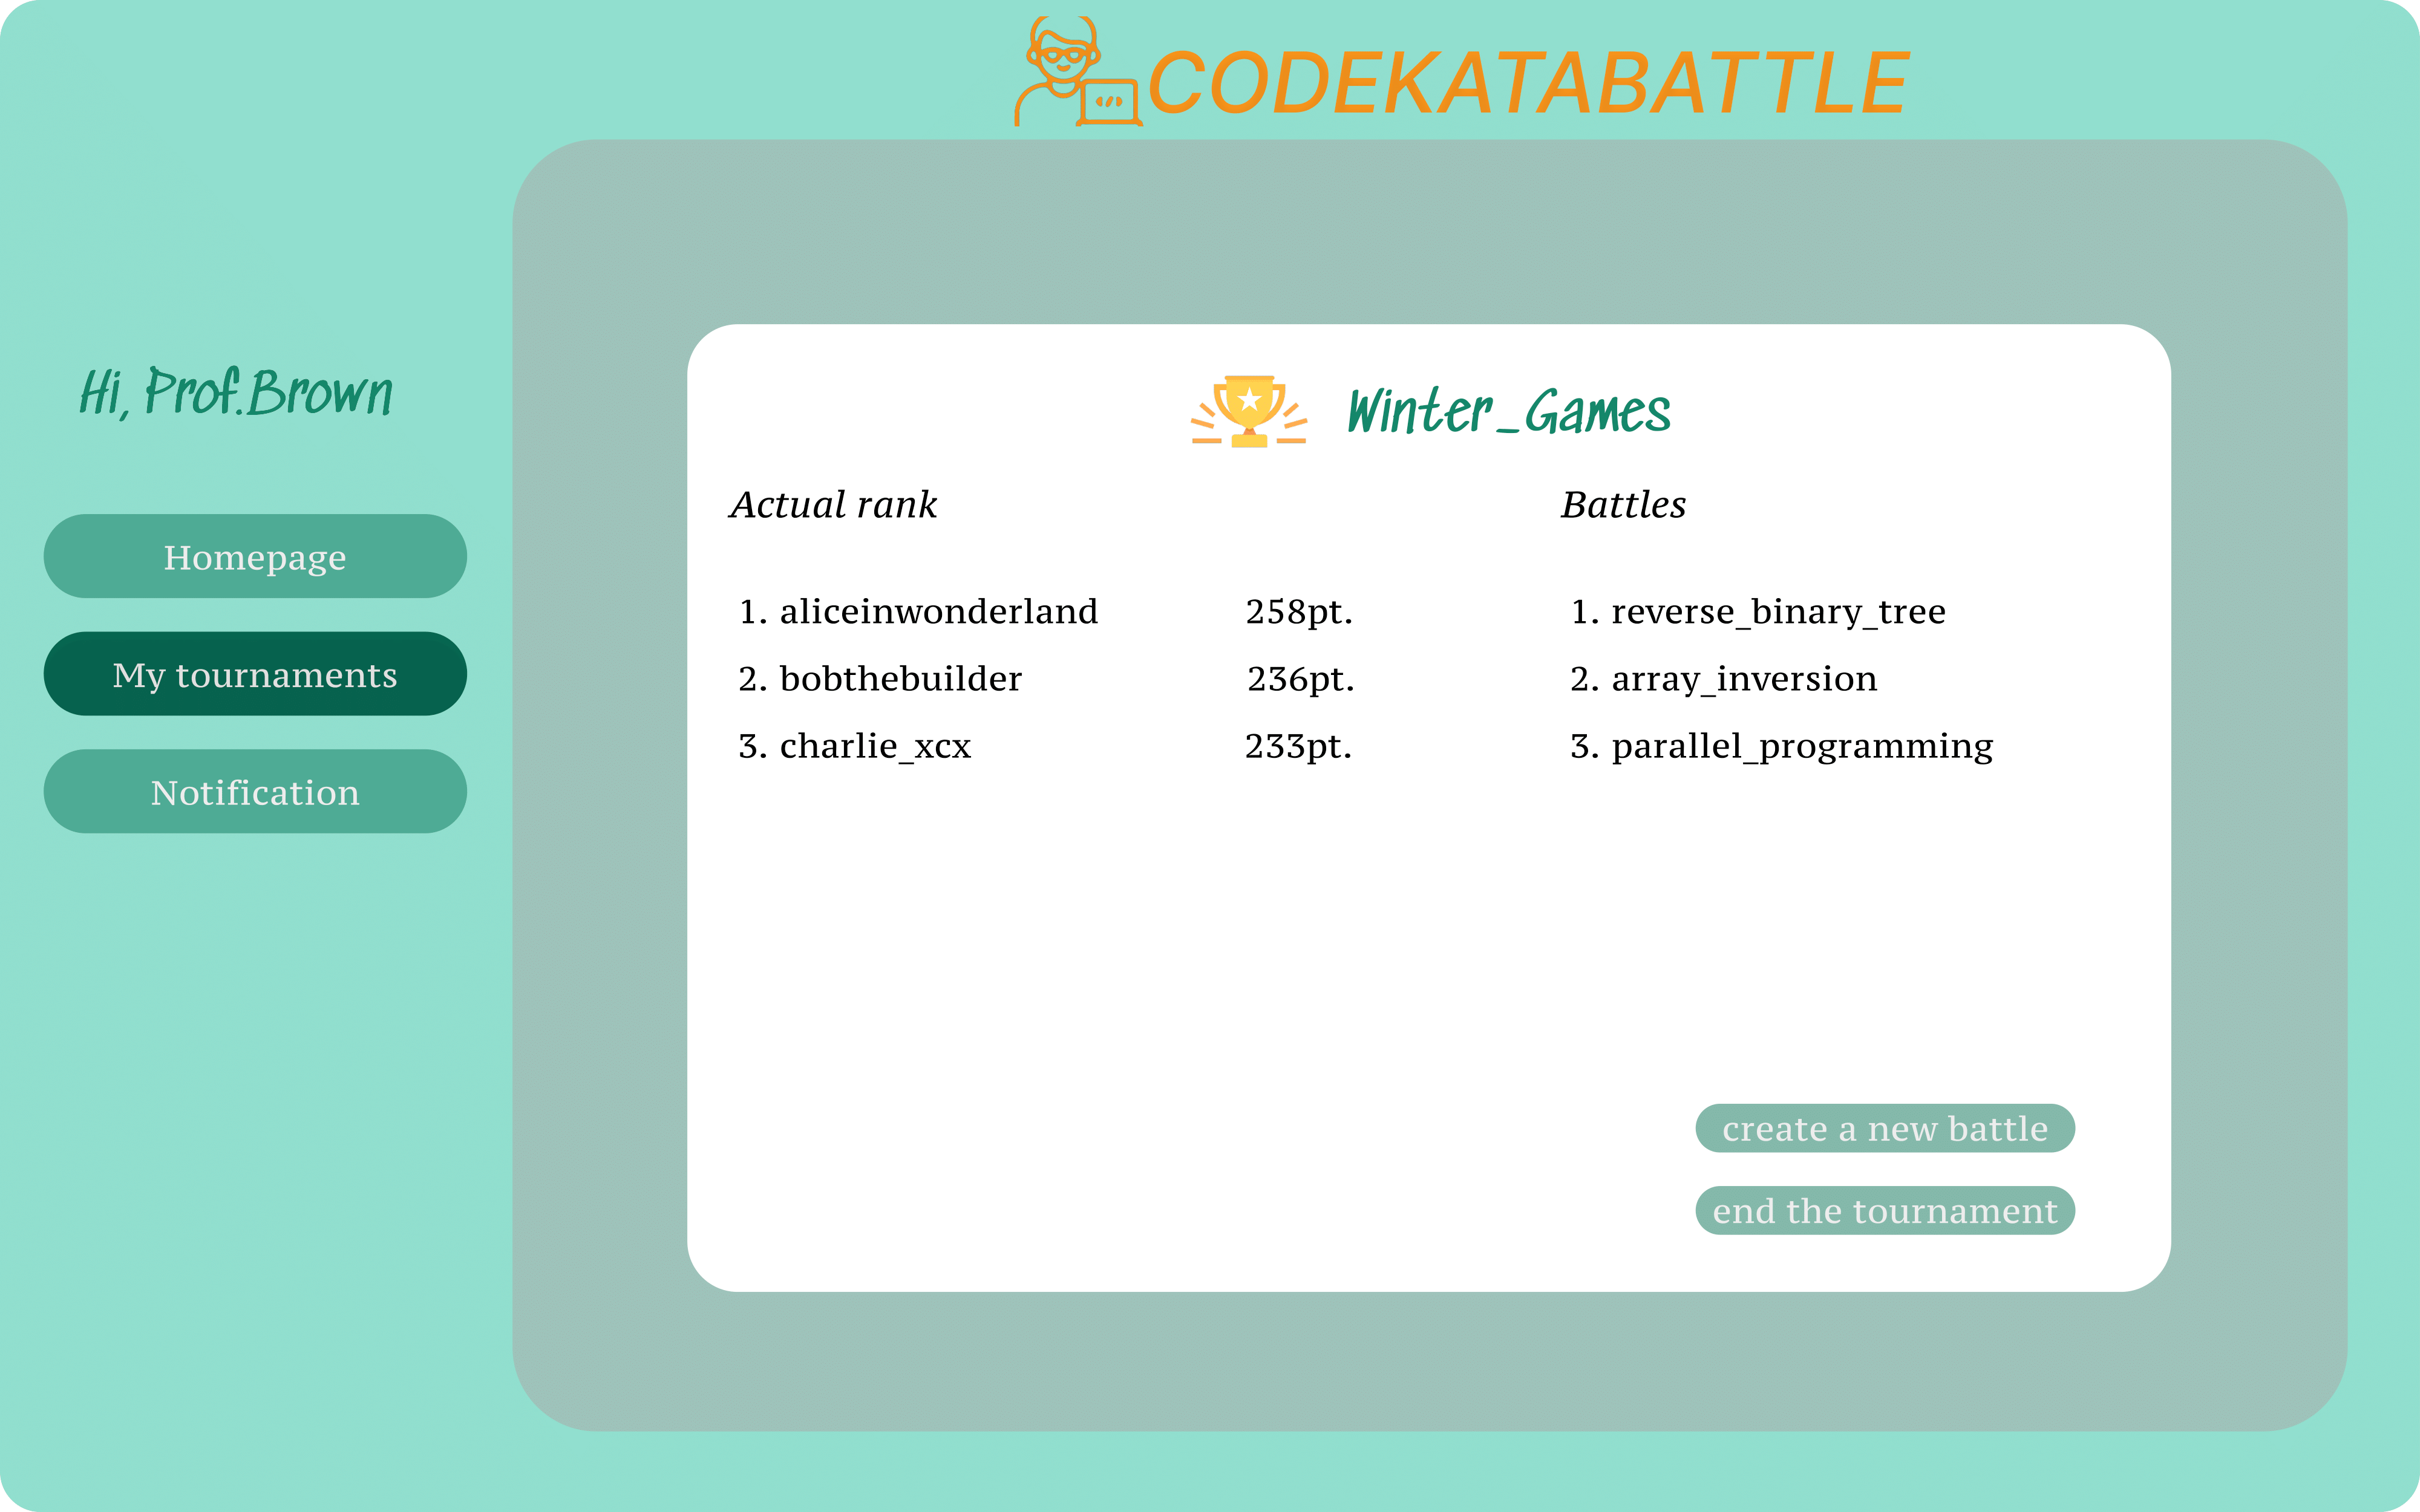
\includegraphics[width=0.8\textwidth]{images/user_interface/UI_sw2-13.png}
    \caption{Tournament's details - educator's page}
\end{figure}

\begin{figure}[H]
    \centering
    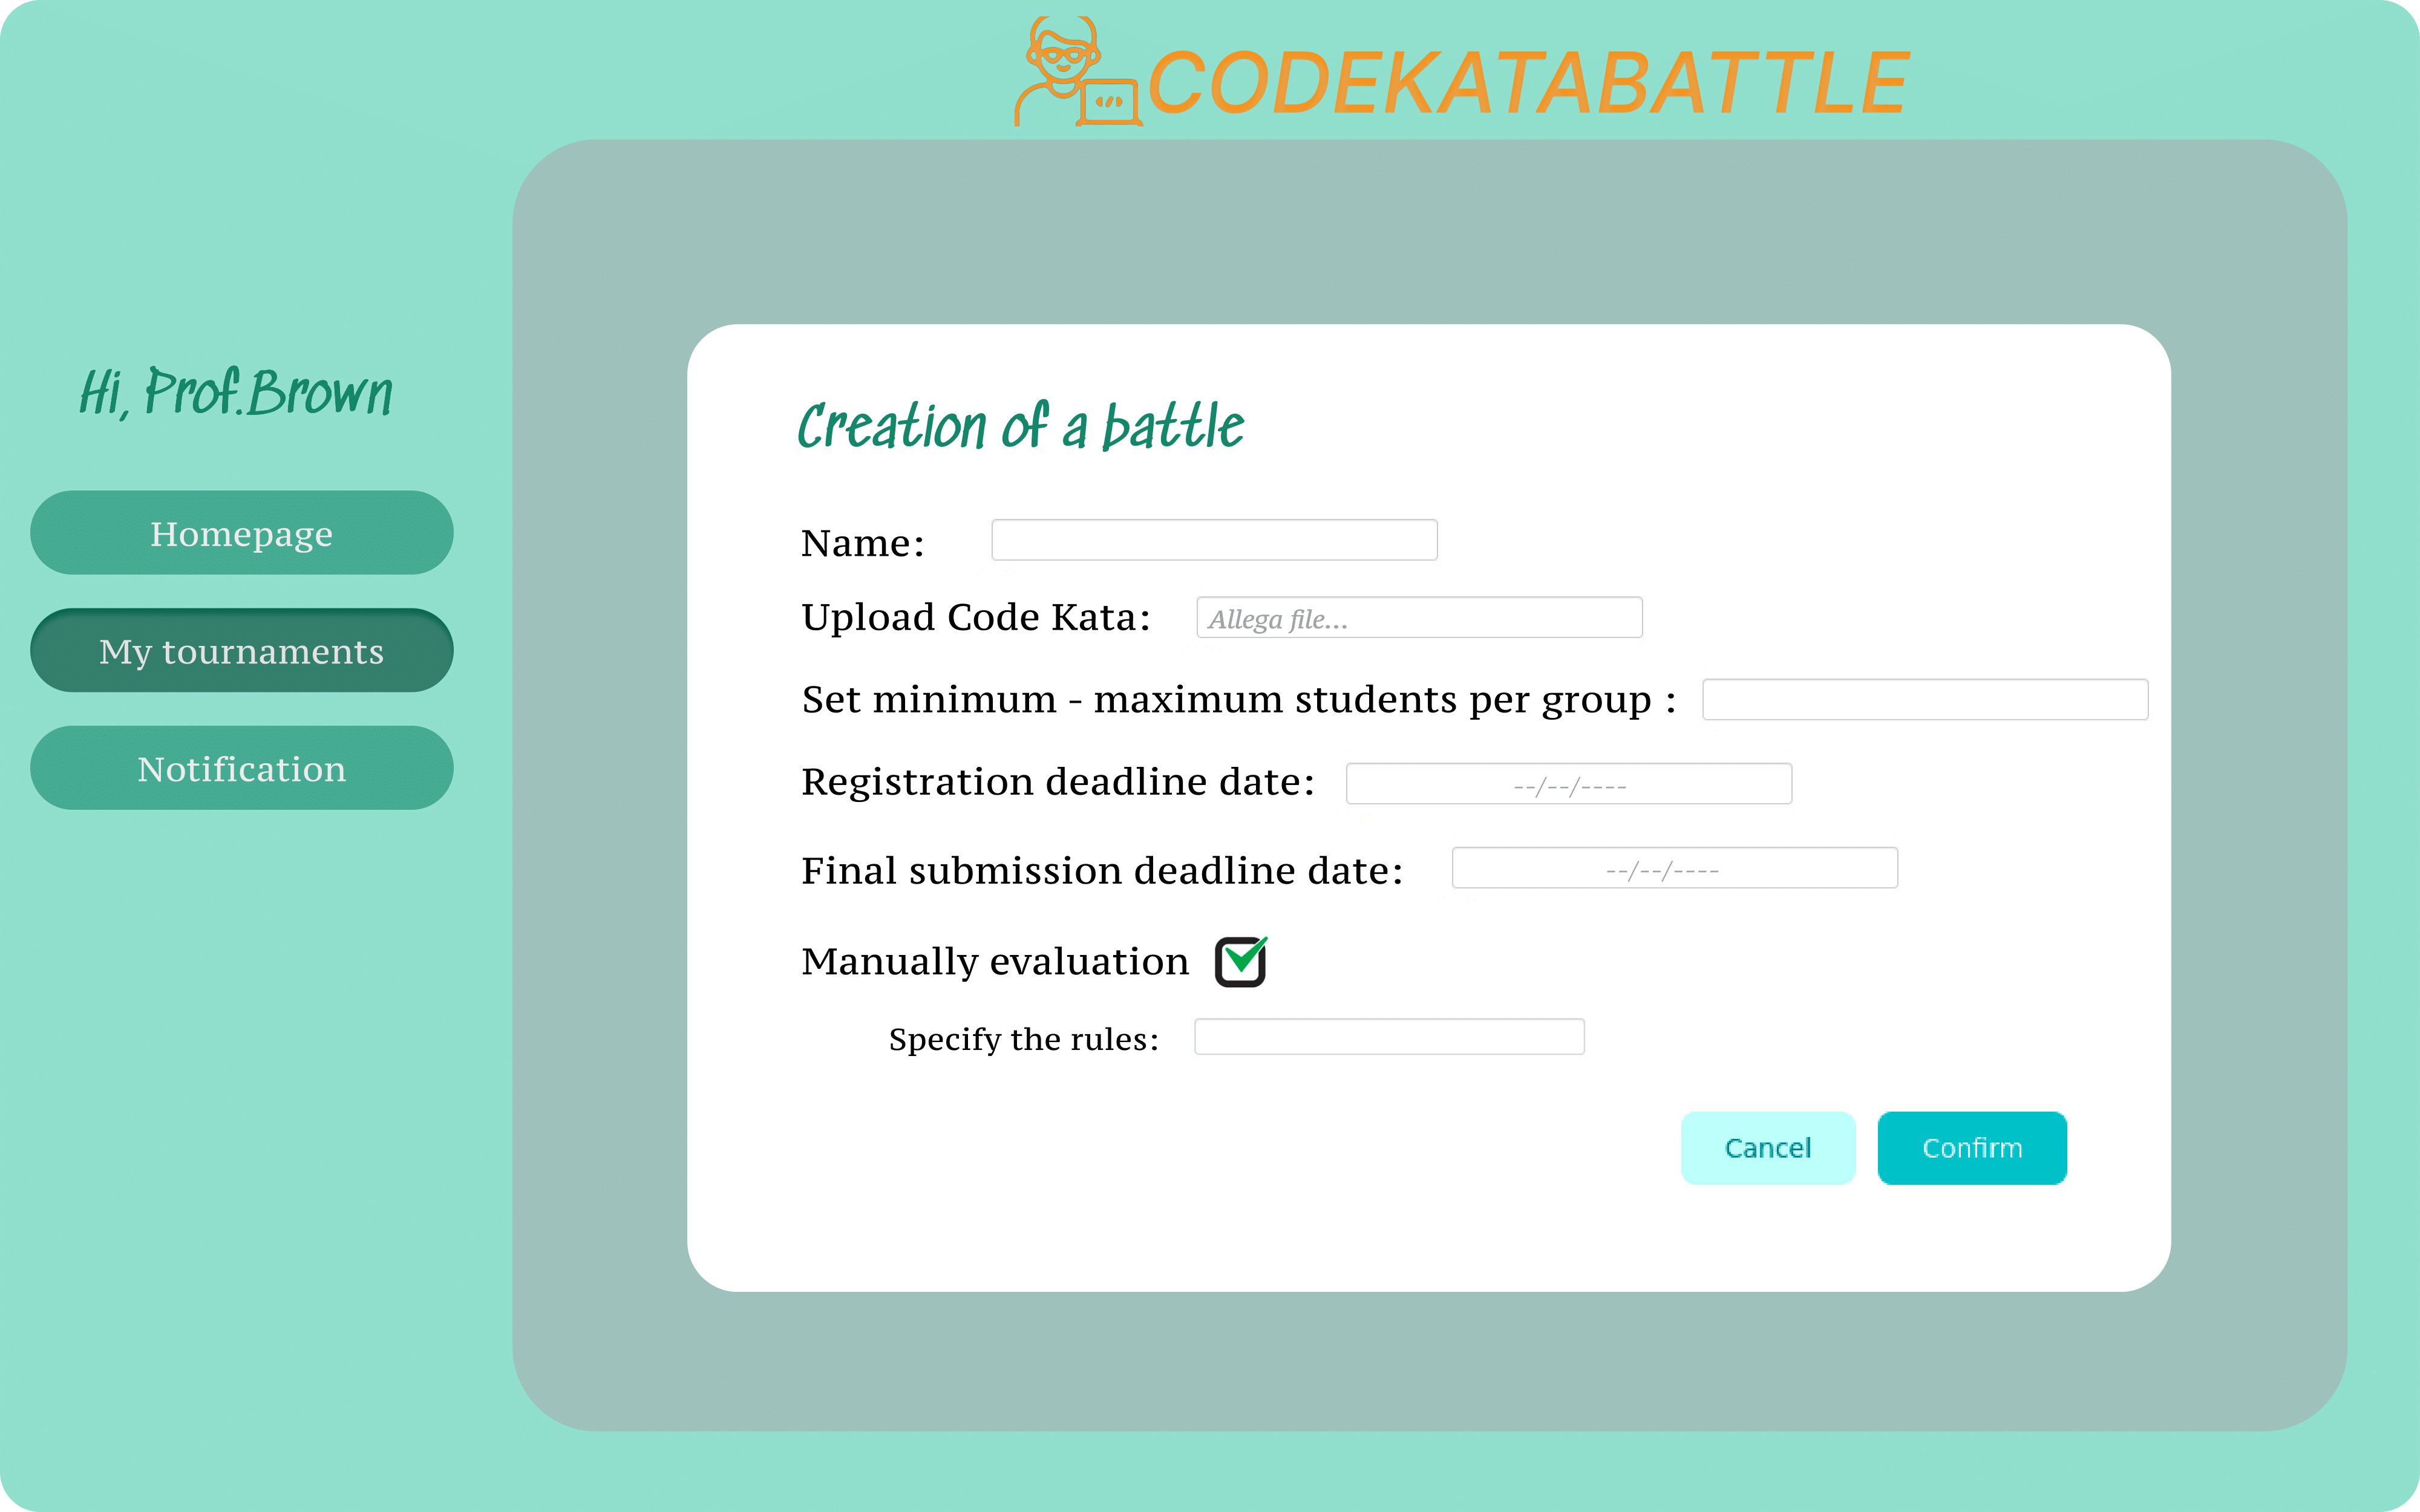
\includegraphics[width=0.8\textwidth]{images/user_interface/UI_sw2-14.png}
    \caption{Creation of a battle page - educator's page}
\end{figure}

\begin{figure}[H]
    \centering
    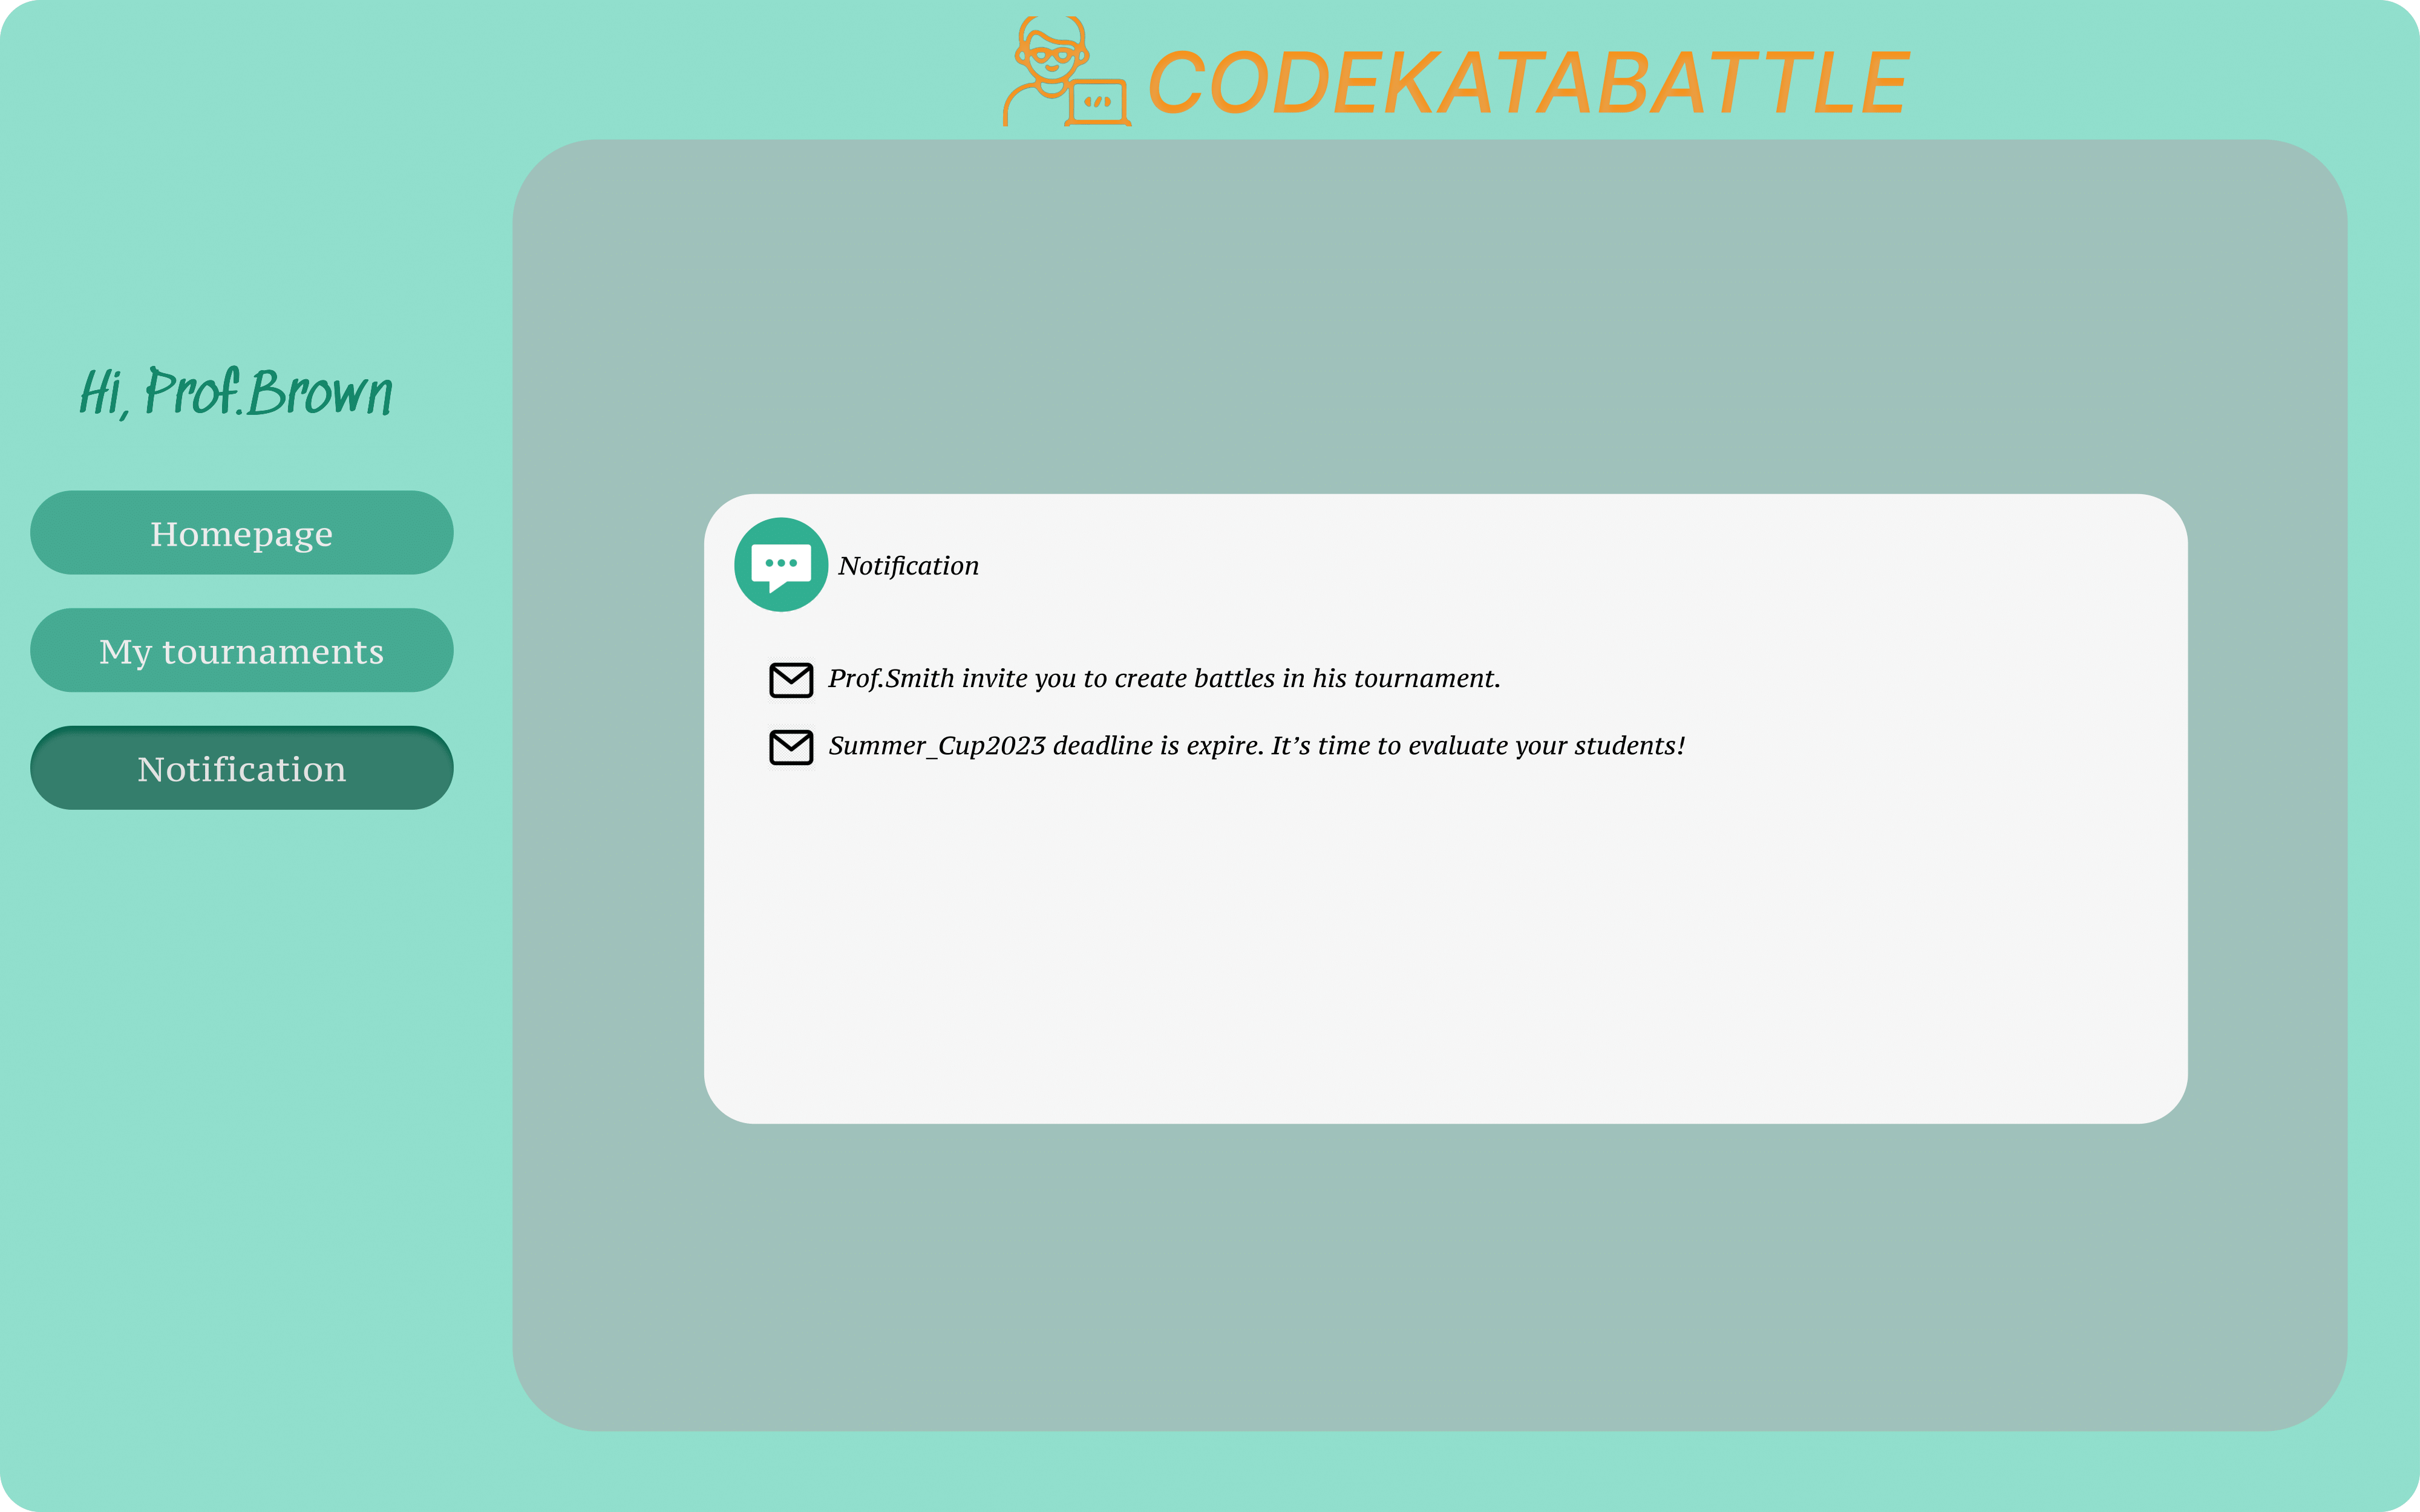
\includegraphics[width=0.8\textwidth]{images/user_interface/UI_sw2-15.png}
    \caption{Notification page - educator's page}
\end{figure}

\begin{itemize}
    \item \textbf{Figure 3.1:} the login page allows registered users (both educators and students) to access the application.
    \item \textbf{Figure 3.2:} the registration page allows new users (both educators and users) to register to the application. They have to specify if they are educators or students.
    \item \textbf{Figure 3.3:} the student's homepage shows the profile of the student and the list of the collected badges.
    \item \textbf{Figure 3.4:} "my tournaments" page shows the list of the tournaments in which the student is enrolled.
    \item \textbf{Figure 3.5:} "tournament's details" page shows the details of the selected tournament. The student can see the actual rank and the completed battles. They can also join a battle, if available.
    \item \textbf{Figure 3.6:} "ongoing tournaments" page shows the list of the tournaments in the platform which deadline isn't already expired. The student can view the details of the tournament.
    \item \textbf{Figure 3.7:} "join a new tournament" page allows the student to join a new tournament. They can visualize the actual rank and the completed battles of that tournament. 
    \item \textbf{Figure 3.8:} "notification" page shows the list of the notifications received by the student. 
    \item \textbf{Figure 3.9:} "submission of a new battle" page allows the student to join a new battle available in the selected tournament . He can read all the details and rules of the battle and, if he want to join, he have to choose the team.
    \item \textbf{Figure 3.10:} the educator's homepage shows the educator's main page.
    \item \textbf{Figure 3.11:} "creation of a tournament" page allows the educator to create a new tournament. He have to specify the name, the description, the deadline, the rules and the granted colleagues. He can also choose to include badges.
    \item \textbf{Figure 3.12:} "my tournaments" page shows the list of the tournaments created by the educator.
    \item \textbf{Figure 3.13:} "tournament's details" page shows the details of the selected tournament to the educator. The educator can see the actual rank and the completed battles. He can also create a new battle, if authorized.
    \item \textbf{Figure 3.14:} "creation of a battle" page allows the educator to create a new battle. He have to specify the name, the code kata, the bound for each team, the final submission deadline. He can also choose to include a manual evaluation.
    \item \textbf{Figure 3.15:} "notification" page shows the list of the notifications received by the educator.
\end{itemize}

\section{User Interface Flow Diagram}
The following diagram shows the connection between the different pages of the application. 
\begin{figure}[H]
    \centering
    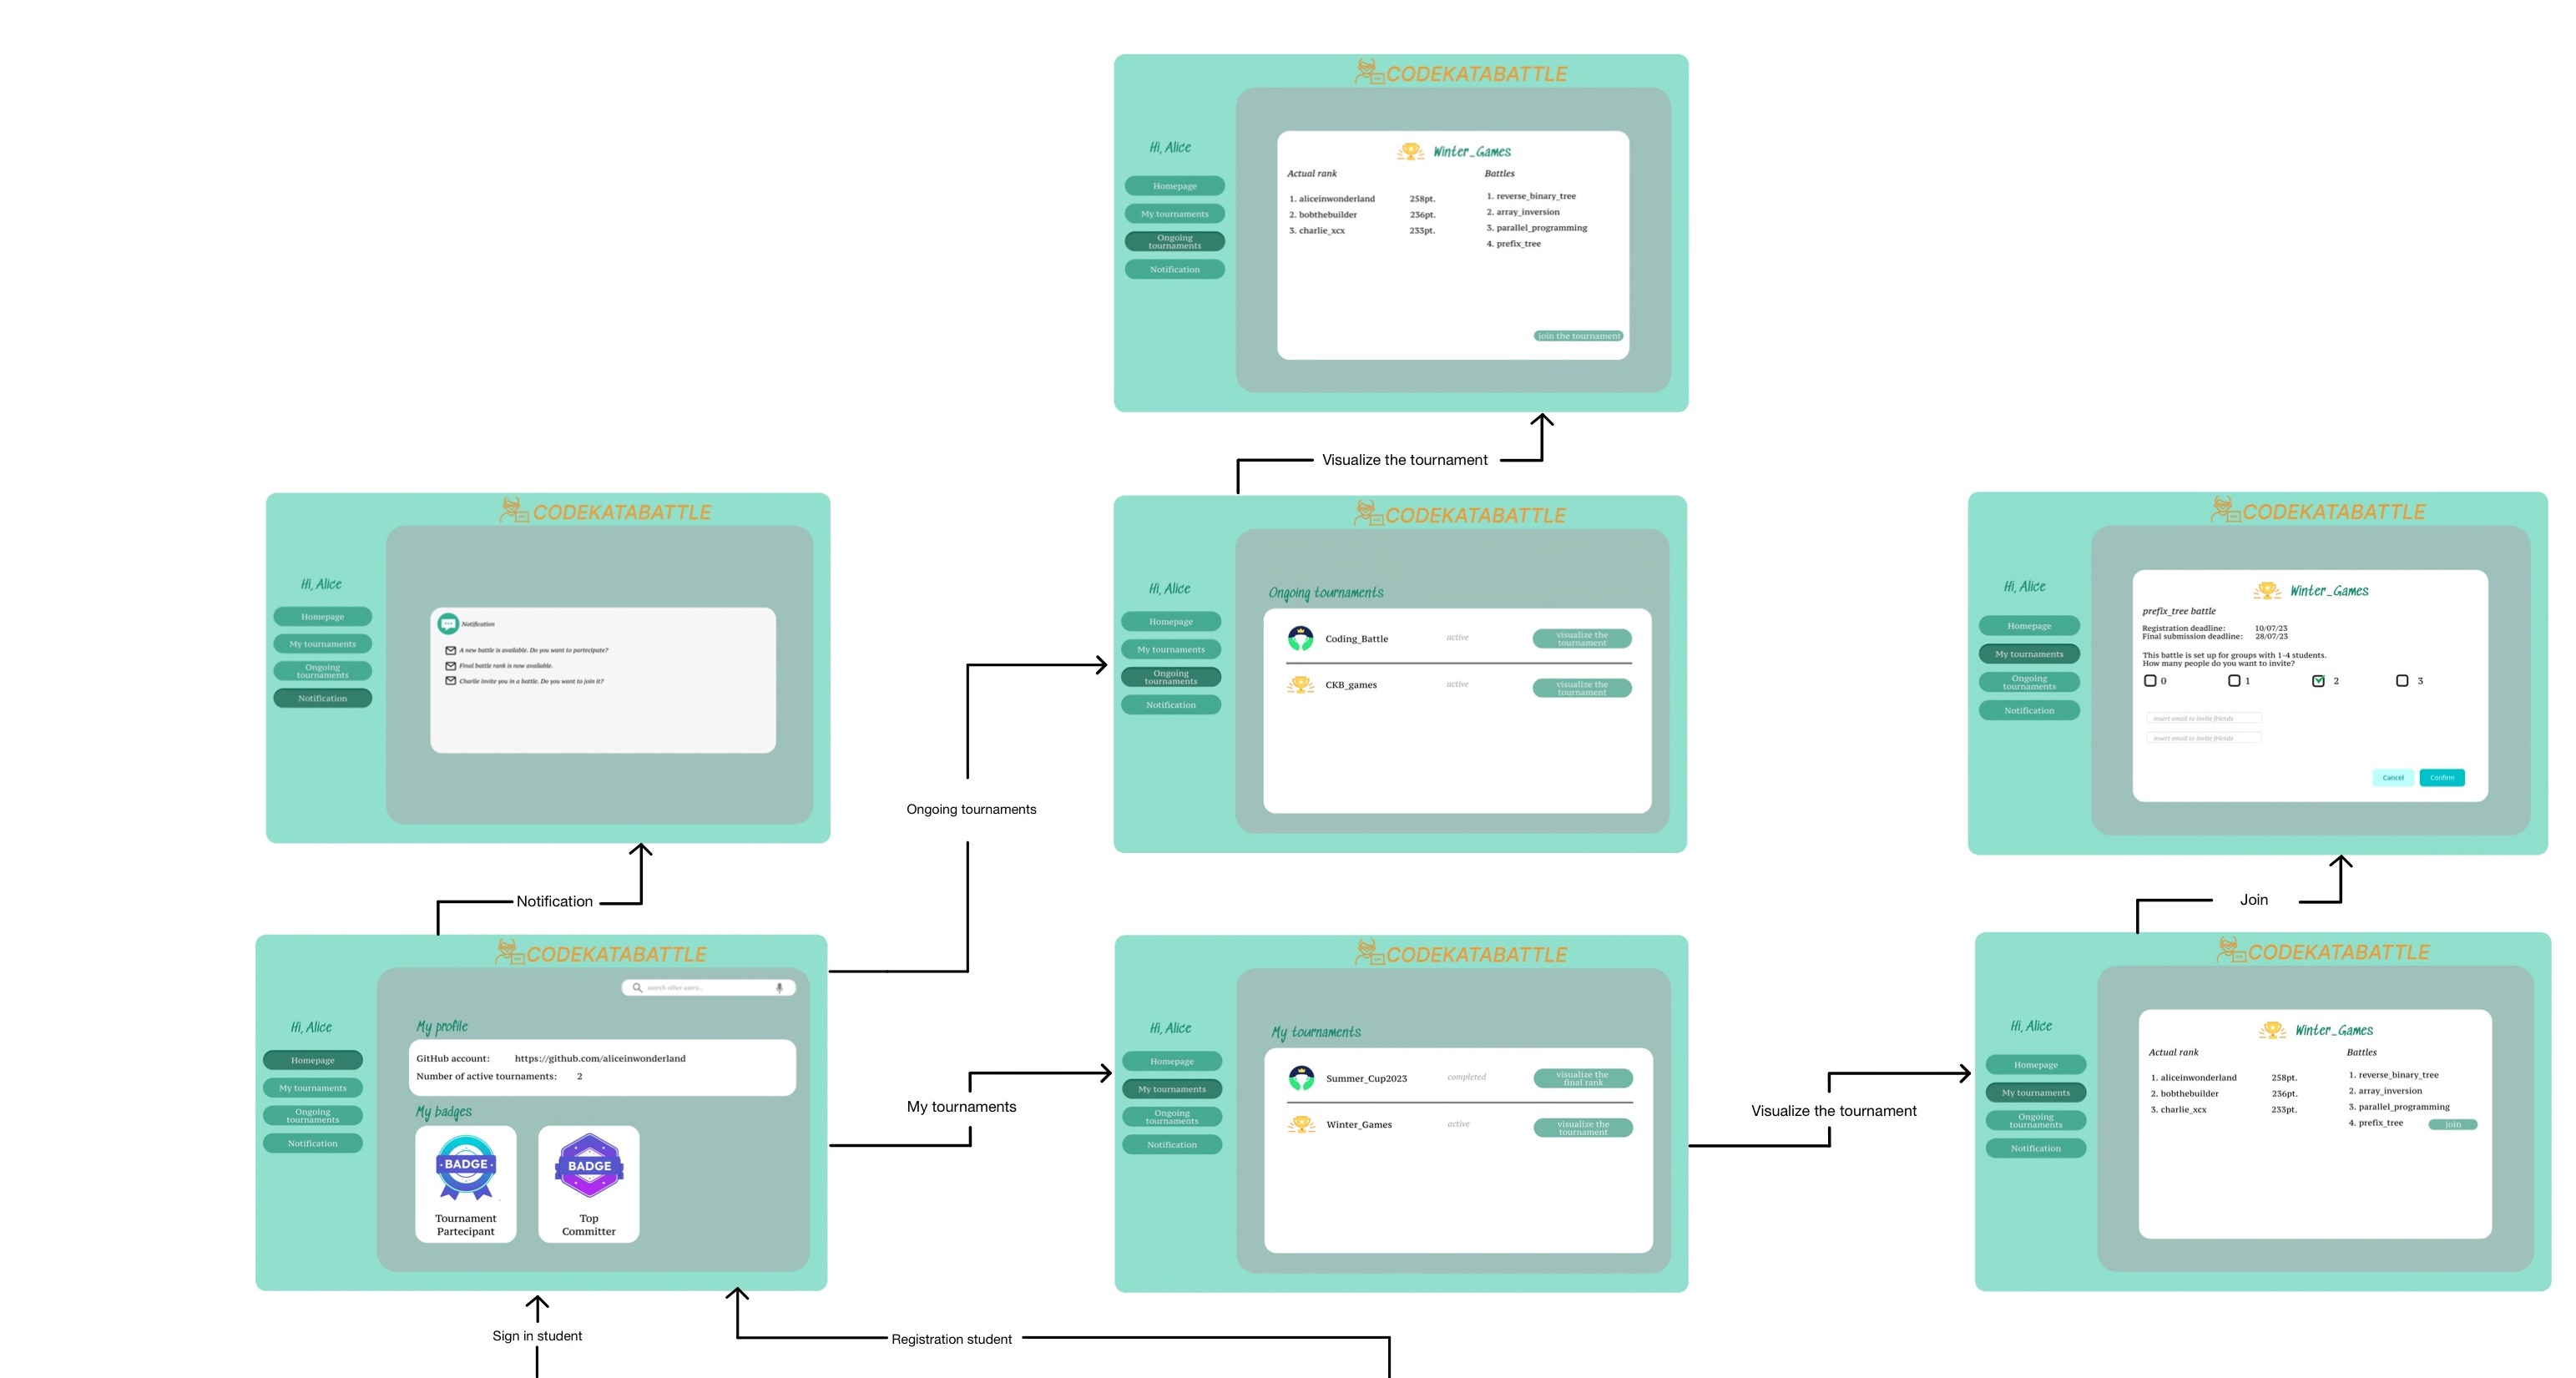
\includegraphics[width=1.15\textwidth]{images/Interface_flow_diagram2.jpg}
    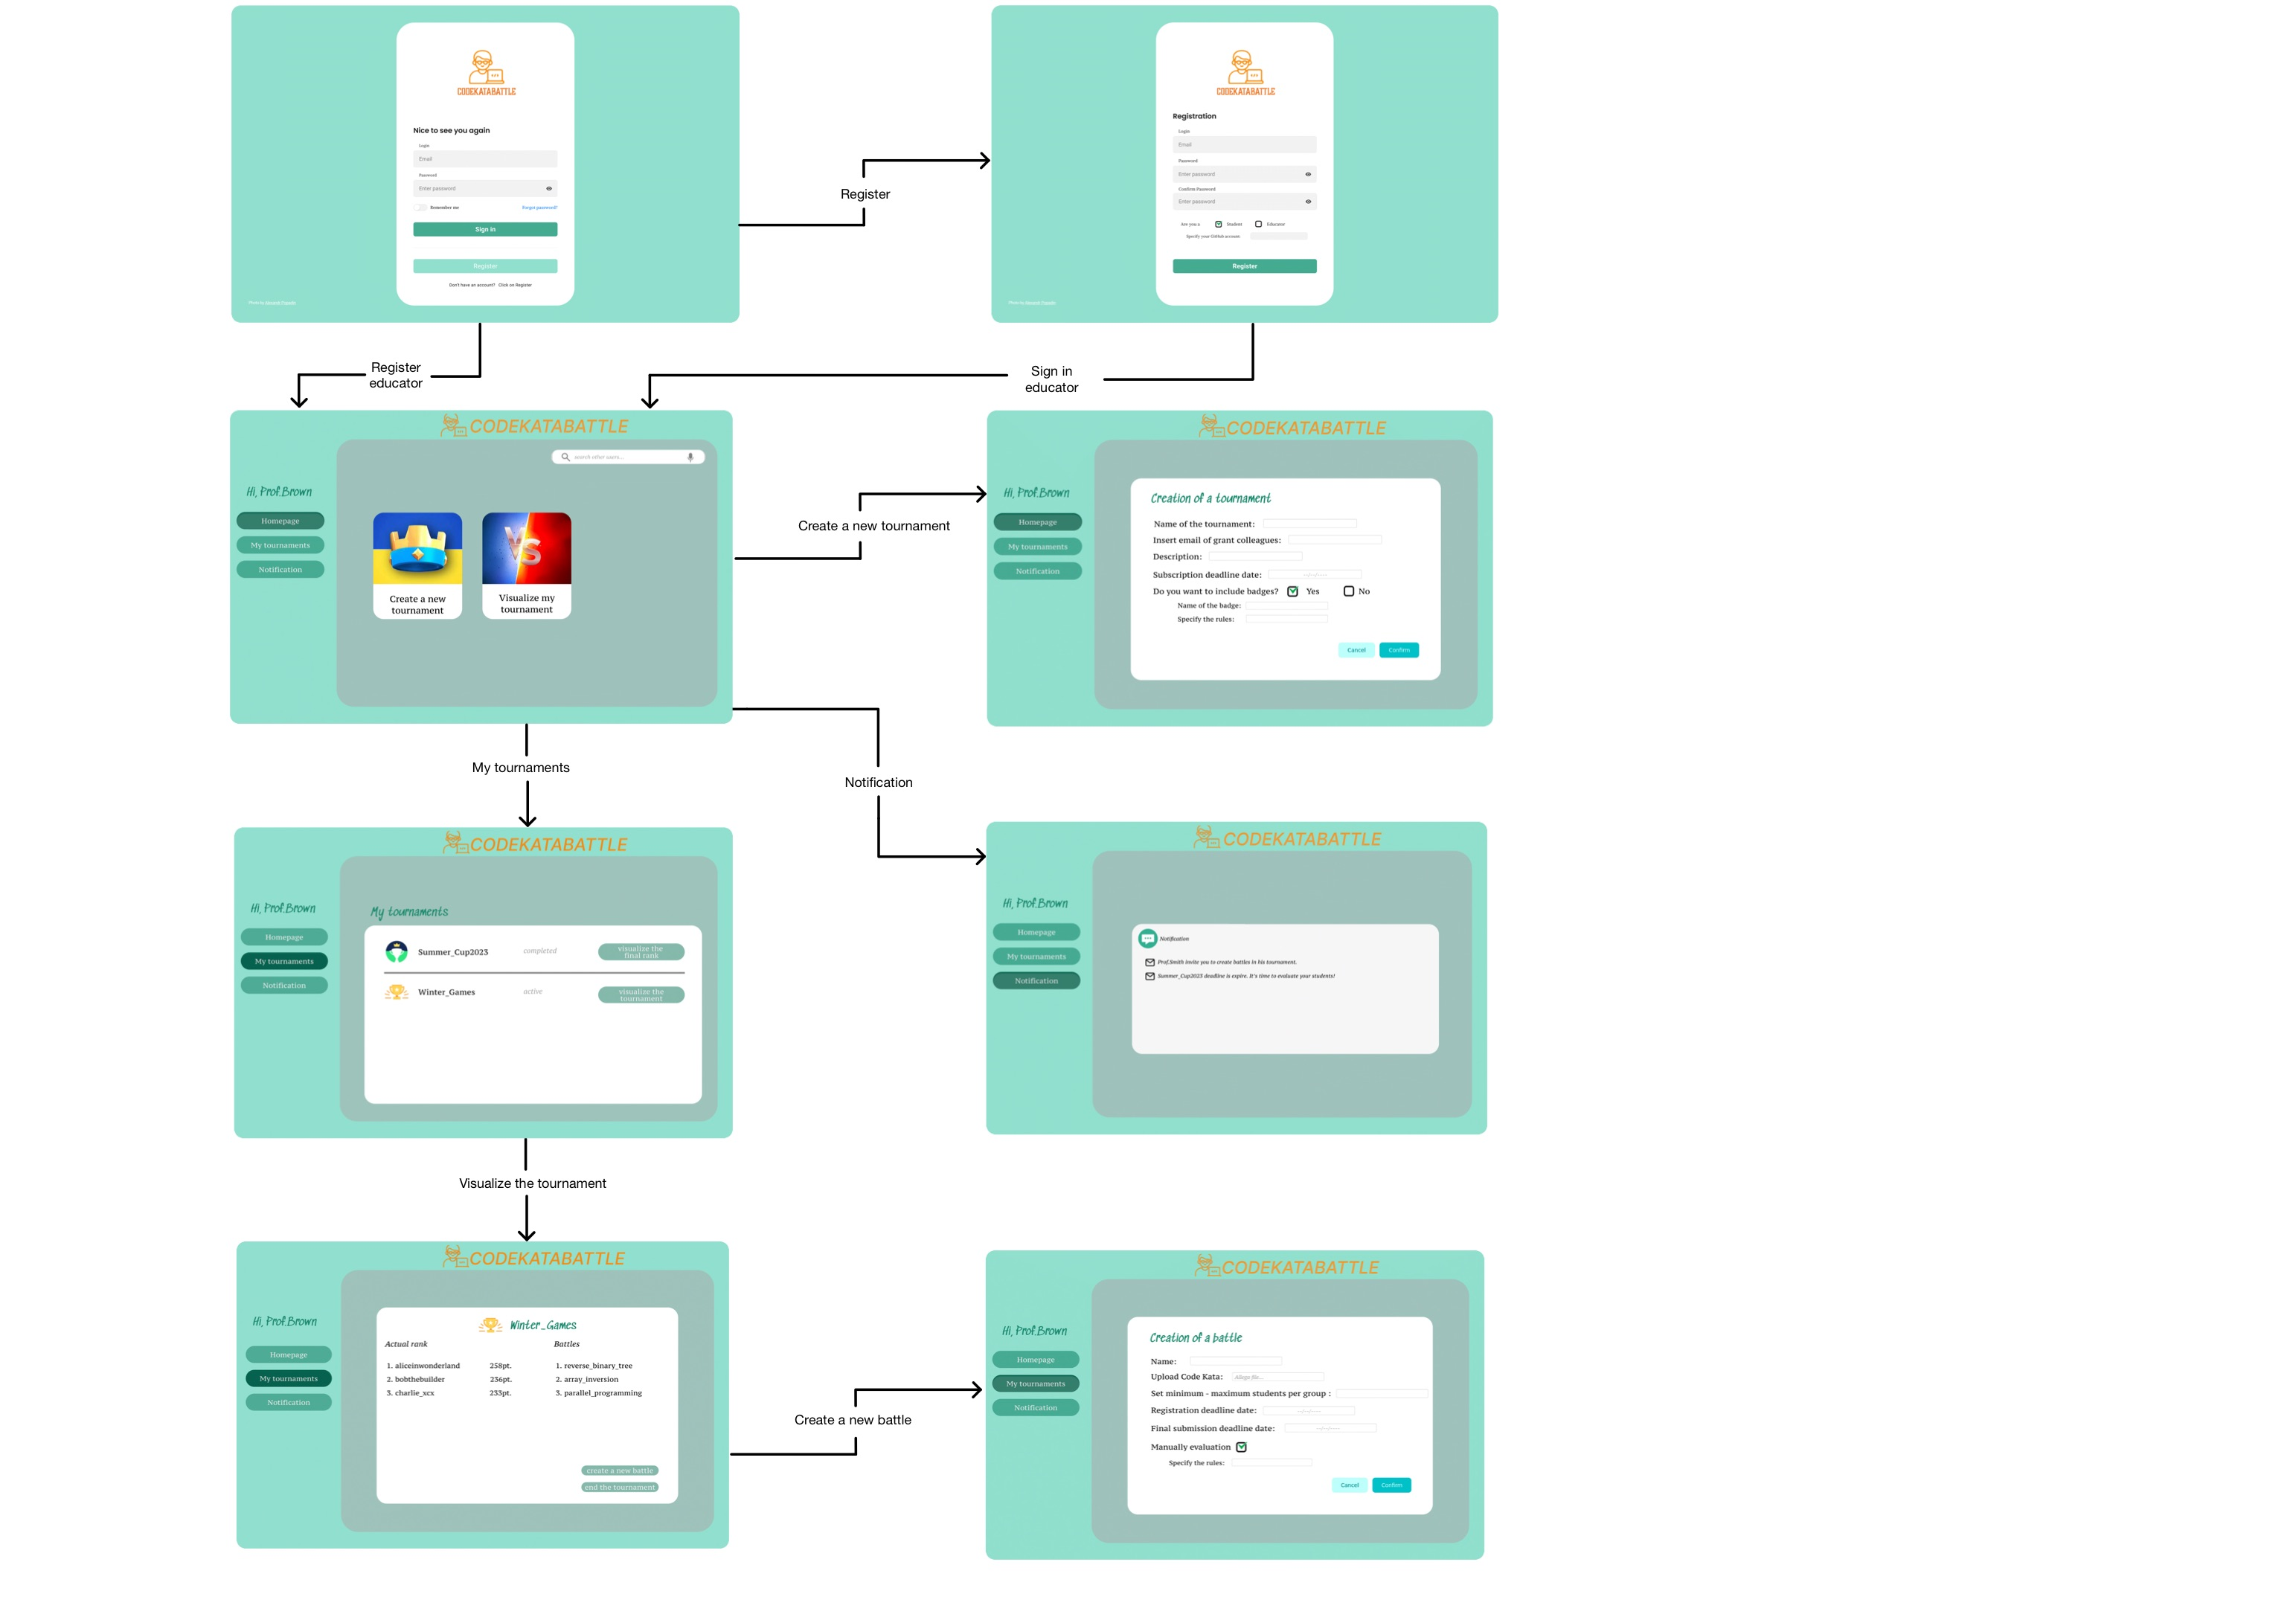
\includegraphics[width=1.15\textwidth]{images/Interface_flow_diagram.jpg} 
    \caption{User Interface Flow Diagram}
\end{figure}